\documentclass[11pt]{book}
\usepackage[utf8]{inputenc}	% Para caracteres en español
\usepackage{amsmath,amsthm,amsfonts,amssymb,amscd}
\usepackage{multirow,booktabs}
\usepackage{titlesec}
\usepackage[Conny]{fncychap}
\usepackage[table]{xcolor}
\usepackage{fullpage}
\usepackage{lastpage}
\usepackage{enumitem}
\usepackage{fancyhdr}
\usepackage{mathrsfs}
\usepackage{wrapfig}
\usepackage{setspace}
\usepackage{calc}
\usepackage{multicol}
\usepackage{cancel}
\usepackage[retainorgcmds]{IEEEtrantools}
\usepackage[margin=3cm]{geometry}
\usepackage{braket}
\usepackage[T1]{fontenc}
\usepackage{pbsi}

\usepackage{pgfplots}
\pgfplotsset{compat=1.15}
\usepackage{mathrsfs}
\usetikzlibrary{arrows}

\usepackage{hyperref}
\usepackage{graphicx}   
\usepackage{geometry}
\usepackage{tikz} 
\graphicspath{{./images/}}

\newlength{\tabcont}
\setlength{\parindent}{0.0in}
\setlength{\parskip}{0.05in}
\usepackage{empheq}
\usepackage{framed}
\usepackage[most]{tcolorbox}
\usepackage{xcolor}
\colorlet{shadecolor}{orange!15}
\parindent 0in
\parskip 12pt
\geometry{margin=1in, headsep=0.25in}
\theoremstyle{definition}

\newtheorem{defn}{Definition}[section]
\newtheorem{exm}{Example}[section]
\newtheorem{example}{Example}[section]
\newtheorem{remark}{Remark}[section]


% FANCY TITLE PAGE
\providecommand{\HUGE}{\Huge}% if not using memoir
\newlength{\drop}% for my convenience
%% specify the Webomints family
%% select a (FontSite) font by its font family ID
\newcommand*{\FSfont}[1]{\fontencoding{T1}\fontfamily{#1}\selectfont}
%% if you don’t have the FontSite fonts either \renewcommand*{\FSfont}[1]{}
%% or use your own choice of family.
%% select a (TeX Font) font by its font family ID
\newcommand*{\TXfont}[1]{\fontencoding{T1}\fontfamily{#1}\selectfont}
%% Generic publisher’s logo
\newcommand*{\plogo}{\fbox{$\mathcal{PL}$}}

\newcommand*{\titlePP}{\begingroup% Printing Poetry
\drop=0.1\textheight
\vspace*{\drop}
\begin{raggedleft}
{Some Lecture Notes for}\\[1.1\baselineskip]
{\bsifamily \HUGE Statistical Mechanics}\\[\baselineskip]
\FSfont{cmr}
{\Large By Moyasui}\par
\end{raggedleft}
\vfill
\begin{center}
\FSfont{cmr}
{\large Spring, 2023}
\end{center}
\vspace*{\drop}
\endgroup}
% FANCY TITLE END

\begin{document}
\pagestyle{empty}
\titlePP
\title{Statistical Mechanics}
\author{Moyasui}
%\maketitle

\tableofcontents
\chapter{Thermodynamics (TD)}
\section{Postulates and Laws}

\begin{itemize}
	\item TD is motivated by applications: steam engines
	\item TD deals with macroscopic equilibrium states.
\end{itemize}

\begin{defn}[Macroscopic state]
	A description of a system based macroscopic measurements. \\
	Temperature, volume, mass, energy, pressure...
\end{defn}
A macroscopic state is not infinitely precise. It doesn't refer to a particle.

\begin{defn}[Equilibrium state]
	A macroscopic state that does NOT change in time. No net transfer of energy or particle or of the system.
\end{defn}

\begin{defn}[State function]
	A function of the small number of quantities that specifies an equilibrium state.
	
\end{defn}

\textbf{Main Assumption:} 
	For every equilibrium state there is a state function called the ENTROPY.

\subsection{Postulates of TD}
\begin{enumerate}
	\item \textbf{Existence of S}:
		\[ S \equiv S(U,V,N). \] 
		The fundamental relation (in the entropy representation) \\
		A macroscopic system has equilibrium states that are characterised uniquely by a small set of extensive variables. \\
		\begin{defn}[Extensive variables]
			Provides a measure of the size of a system. Answer ``how much`` questions. (U: energy, V:Volume, N:Number of particle (mass).)
		\end{defn}
		The fundamental relation gives all TD info about the system. (because you can invert the equation above to get U,V,N)
	\item \textbf{Maximisation:} The values of the extensive variables of an isolated system in the absence of an internal constraint are those that maximise the entropy over the set of all constrained macroscopic states.
		\begin{figure}[htpb]
		\begin{center}
		\begin{tikzpicture}[scale=1, transform shape]
			
			
		\end{tikzpicture}
		\end{center}
		\caption{Box with removable wall.}%
		\label{fig:postulate2}
		\end{figure}
		We have then:
		\[
		S(U_A,V_A,N_A,U_B, V_B,N_B) \]
		\[U=U_A+U_B\] same for $ V,N $ 
		Removing wall, the values of $ U_A, V_A, N_A $ will be such that it maximises $ S$. 
	\item \textbf{Additivity}:
		The entropy of a composite system is additive over its constituent subsystems.
		\[S(X_A, X_B) = S(X_A) + S(X_B)\]
		This is not true if there exist long range forces but usually well satisfied.\\
		Hold whenever interactions between particles are much shorter than the system size.
	\item \textbf{Continuity and Differentiability:} 
		The entropy is a continuous and differentiable function of the extensive parameters.
	(NOT true at phase transitions.)
	\item \textbf{Extensivity:}  
		The entropy is an extensive function of its extensive variables.
		\[ S(\lambda U, \lambda V, \lambda N) = \lambda S(U,V,N) \quad \lambda \in \mathbb{R}\] 
		(Only holds if surface effects can be neglected.)
	\item \textbf{Monotonicity:}
		The entropy is a monotonically increasing function of energy for equilibrium volumes of the energy.
		\[ \frac{\partial S}{\partial U} \vert _{V,N} > 0\] 
		(Something funny happens at negative temperature.)
	\item \textbf{Nernst postulate:} The entropy of any real physical system is non-negative.(Only applies to QM systems. Doesn't apply to f.eks ideal gas.)
\end{enumerate}

\begin{defn}[Temperature in TD]
	\[ \left( \frac{\partial S}{\partial U} \right) \vert _{N,V} \equiv \frac{1}{T}  \] 
	
\end{defn}

\subsection{TD laws}
\begin{itemize}
	\item If two systems are in equilibrium with a third system, they are also in equilibrium with each other. (Their intensive variables are equal)
	\item Heat is energy and energy us conserved.
	\item After the release of a constraint in a closed system, the entropy never decreases.
	\item The entropy of a quantum mechanical system goes to a constant as $ T \to 0 $.
\end{itemize}

0th law:
It follows from P.2(maximisation) and P.3(additivity).
\[ S = S(U_A, V_A, N_A) + S(U_B, V_B, N_B) \] 
\[ U_B = U - U_A \] 

*Caclulations* 

 \section{Small Changes: Inexact and exact differentials}
 Consider a function of $ 2 $ variables $ F(x,y) $ 
 The differential of this is:
 \begin{equation}
 	df = \left (\frac{\partial f}{\partial x} \right )_y dx + \left (\frac{\partial f}{\partial y}\right )_x dy 
 \end{equation}
 This is an exact differential. \\
 Exact differential gives a \textbf{unique (does not depend on the integration path)} function (up to a constant) when integrated.

 \[ \int_{{(0,0)}}^{{(x,y)}} {df} = \int_{{(0,0)}}^{{(,y)}} { \frac{\partial f}{\partial y} } \: d{y} + \int_{{(0,y)}}^{{(x,y)}} { \frac{\partial F}{\partial x} } \: d{x} \]
\begin{shaded*}
	Condition for exact differential:
	\[ \left( \frac{\partial f}{\partial y}\right)_x  = \left( \frac{\partial g}{\partial x}\right)_y\] 
\end{shaded*}
\begin{large}
	\textbf{But not every differential} 
\end{large}
\[ \text{\dj} f = f(x,y) dx + g(x,y)dy \] is exact
For instance:
\[ \text{\dj} F = -ydx+xdy \] is not exact.
 (The integral is path dependant.)
 \[ \int_{(0,0)}^{(x,y)} \not dF = \int_{(0,0)}^{(x,0)} -ydx + \int_{(x,0)}^{(x,y)} xdy = xy, \]  
 \[ \int_{(0,0)}^{(x,y)} \not dF = \int_{{(0,0)}}^{{(0,y)}} {x} \: d{y} + ...
  \]  
Not the same. \\
\begin{shaded*}
	We can always find an integrating non unique factor (function) so that
	\[ dG = r(x,y)\not dF \] 
\end{shaded*}

For \[ \text{\dj} F = -ydx+xdy \]
want 
\[ dG = (-r(x,y)y)dx + (r(x,y)x) dy\] 
$ r = \frac{1}{xy} $ 

This is the same thing as used when solving first order diff.equation. \\

Next: work and heat are not exact. 

Conservation of energy:
$ dU = \text{\dj} Q \text{(Heat added)} + \text{\dj} W \text{(work done \textbf{on} the system)}$
$ U $  is a state function so $ dU $ is exact.
$ \text{\dj} Q $ and $ \text{\dj} W $ are inexact as they cannot be derived.   

\subsubsection{Work}%
\label{ssub:Work}

\begin{equation}
	\text{\dj} W = \vec{F_{outer}} \cdot d \vec{x} > 0
\end{equation}
\[ F_{outer} = - F_{inside} \] 
\[ \text{\dj} W = -F_{inner} \cdot dx \] 
\[ \text{\dj} W = -pdV \] 
\[ -\frac{1}{p} \text{\dj} W = dV \] 
Here $ -1/p $ plays the role of an integrating factor.

\[ \int_{(0,0)}^{(p,v)} = \int_{(0,0)}^{p,0} + \int_{(p,0)}^{p,V} -p dV = -pV\] 
\[ \int_{(0,0)}^{(p,v)} = \int_{(0,0)}^{(0,v)} -pdV = 0   \] 
\textbf{Path dependant} 
work can also be magnetic or electric.
\subsubsection{Heat}%
\[ dS = S(U+\text{\dj} Q, V, N) - S(U,V,N) \] 
\[ = \left( \frac{\partial S}{\partial U} \right)_{(v,N)} \text{\dj} Q  \] 
\[ \implies \text{\dj} Q = T dS \] 

\[ dS = \frac{1}{T} \text{\dj} Q \] 

\subsubsection{Conservation of energy}%
\label{ssub:Conservationofenergy}
$ dU = \text{\dj} Q + \text{\dj} W $ 
\[ dU = T dS - pdV \] (N const)
\[ U = U(S,V,N) \] 
\[ dU = \left ( \frac{\partial U}{\partial S}\right )_{V,N} dS + \left ( \frac{\partial U}{\partial V}\right )_{S,N} dV + \left( \frac{\partial U}{\partial N}\right )_{S,V} dN \] 
\[ \left(\frac{\partial U}{\partial S}\right)_{V,N} = T \] 
\[ \left(\frac{\partial U}{\partial V}\right)_{S,N} = -P \] 
\[ \left(\frac{\partial V}{\partial N}\right)_{(S,V)} \equiv \mu \] 
With N varying:
\begin{shaded*}
\[ dU = TdS - PdV + \mu dN \] 
\end{shaded*}
In entropy representation:
	\[ S = S(U,V,N) \] 
	\[ dS = \left(\frac{\partial S}{\partial U}\right)_{(V,N)} + \left(\frac{\partial S}{\partial V}\right)_{U,N} dV +
	\left(\frac{\partial S}{\partial N}\right)_{U,V} dN\] 	
\begin{shaded*}
	\[ dS = \frac{1}{T} dV + \frac{P}{T}dV - \frac{\mu}{T}dN \] 
\end{shaded*}
\subsection{TD Processes}
For all processes in a closed system, \[ dS \geq 0 \] 
$dS = 0 $ when system is already in equilibrium. \\
Processes when $ dS > 0 $ in termed irreversible.
\subsubsection{Quasistatic process}%
\label{ssub:Quasistaticprocess}
\begin{defn}
	In the limit of infinitesimal changes at an equilibrium system (very slow ideal process)
	\[ \Rightarrow dS = 0 \] 
	
\end{defn}
It's an idealisation, doesn't exist.

\subsubsection{Heat Engines}%
\label{ssub:HeatEngines}
Produce work from heat (steam engine).

Such engines are cyclic, 
\[ dU = 0, \quad dS = 0, \quad  dV = 0, \quad dN = 0\] in a cycle.
\[ dU = 0 \implies \text{\dj} Q + \text{\dj} W = 0 \] 
\[ \implies - \text{\dj} W = \text{\dj} Q \] 

\[ dS = 0 \] 
\[ T \text{\dj} Q = 0 \] 
This shit doesn't do any work, new engine:
Need a hot and a cold reservoir (to dump heat)
\[ \frac{\text{\dj} Q_i}{T_i} - \frac{ \text{\dj} Q_o}{T_o} = 0 \] 
\[ \implies \text{\dj} Q_o = \frac{T_i}{T_o} \text{\dj} Q_i \] 
\[ \text{\dj} Q_i - \text{\dj} Q_0 +\text{\dj} W  = 0\] 
\[ \implies -\text{\dj} W = \text{\dj} Q_i (1-\frac{T_o}{T_i}) \] 
\textbf{Efficiency} 
\[ \eta = \frac{-\text{\dj} W}{\text{\dj} Q_i} = 1 - \frac{T_o}{T_i} = \frac{T_i - T_o}{T_i} \] 

\subsubsection{Fridge and Air conditioners}%
\label{ssub:Fridge and Air conditioners}

Diagram\\
Fridges are heat engines run in reverse.
\[ \text{\dj}W + \text{\dj}Q_I - \text{\dj}Q_o = 0 \quad (dU = 0)\] 
\[ \frac{ \text{\dj} Q_I }{T_I} - \frac{ \text{\dj}Q_o }{T_o} \quad dS=0 \] 
Coefficient of Performance is 
\[ COP_{cooling} = \frac{- \text{\dj}Q_o}{ \text{\dj}W }\] 
\[ \implies \text{\dj}Q_I = T_I \frac{ \text{\dj}Q_o }{T_o} \] 

\[ \left( \text{\dj}W + (\frac{T_I}{T_o} - 1) \text{\dj}Q_o \right)  = 0\] 
Reduce efficiency as $T_o \to 0$.

\subsubsection{Heat Pumps}%
\label{ssub:Heat Pumps}
Same as refridgerators, but inside of fridge is outside of the house.

\[ COP_{heating} = \frac{ \text{\dj}Q_I }{ \text{\dj}W } = \frac{1}{1-\frac{T_o}{T_I}} = \frac{T_I}{T_I-T_O} \] 
with \[ \text{\dj}Q_O = \frac{T_o}{T_I} \text{\dj}Q_I \] 
\[ \text{\dj}W + \text{\dj} Q_I - \frac{T_o}{T_I} \text{\dj}Q_I = 0 \] 
\[ \text{\dj}W = \text{\dj}Q_I \left( \frac{T_O}{T_I} - 1 \right)  \] 

For a non-reversible engine:
\[ dS =\frac{ \text{\dj}Q_I}{T_I} - \frac{ \text{\dj}Q_O}{T_O} + \text{\dj}A \] 

$ A $ is the positive entropy generated in a cycle.

\section{TD Potentials}
Fundamentlal relation:
\[ S=S(U,V,N) \text{or} U=U(S,V,N) \] 
from this we can derive all TD.

\begin{exm}[Ideal Gas]
	\[ S = Nk_B\left( \frac{3}{2}ln(\frac{V}{N}) + ln (\frac{V}{N}) + ln X \right)  \] 
	where $ X $ is independent of $ U,V,N $ 
	
	\[ \frac{1}{T} = \frac{\partial S}{\partial V}_{V,N} = \frac{3}{2}Nk_B \frac{1}{U} \] 
	\[ \implies U = \frac{3}{2}Nk_bT \] 
	\[ \frac{P}{T} = \frac{\partial S}{\partial V}_{V,N} = \frac{Nk_b}{V} \] 
	\[ \implies PV = Nk_BT \] 
	\[ -\frac{\mu}{T} = \frac{\partial S}{\partial N}_{U,V} = \frac{S}{N} - Nk_B \frac{5}{2}\frac{1}{N} = \frac{S}{N}-\frac{5}{2}k_B\] 
	\[ \implies S = \frac{5}{2}k_BN - \frac{\mu N}{T} \] 
	These are all equations of states, not fundamental relations.
\end{exm}
	
\textbf{How can we extract TD info at constant $ T,P $ etc. ?} 
\[ T = \frac{\partial U}{\partial S}_{V,N} - \frac{\partial U}{\partial V}_{S,N}\] 

\subsection{Legendre Transform}
Given $ y = y(x) $ let's call $ \frac{\partial y}{\partial x} = p $ 
\[ \tilde y(p) \] 
Try $ \tilde y = y $ and make a table. \\
\begin{table}[htpb]
	\centering
	\begin{tabular}{c c}
		p & y \\
		... & ...
	\end{tabular}
\end{table}
Useless, no way to know where on the x-axis.\\
Second try: replace $ \tilde y $ by the y-intercept of the curved tangent.
This works, but requires $ \frac{\partial y}{\partial x} $ monotonic (as temperature is).

\[ y- \tilde y = px \] 
\[ \tilde y = y - px \] 
\begin{exm}
	\[ y=x^2 \] 
	\[ p = \frac{\partial y}{\partial x} = 2x \implies x = \frac{p}{2} \] 
	\[ \tilde y(p) = y - px = x^2 - px = \frac{p}{2}^2- p \frac{p}{2} = - \frac{p^2}{y} \] 
	Inverse: 
	\[ y(x) = \tilde y + px = - \frac{p^2}{y} + px = \frac{-(2x)^2}{y} + 2x^2 = x^2 \] 
\end{exm}

Differentials:
\[ d \tilde y = dy - pdx - dp x = -x dp \] 
\[ dy = d \tilde y + x dp + p dx = p dx \] 
Switches and negative.

\subsection{Helmholtz free energy}
\[ U=U(S,V,N) \] want a function of $ T,V,N $ that gives all TD info.
\[ T = \frac{\partial U}{\partial S}_{V,N} \] 
\[ F = U - TS \] eliminate  $ U,S $ in favour of $ T,V,N $ 
\[ = F(T,V,N) \] (is a fundamental relation.)
\[ dF = dU-TdS - sdT \] 
recall $ dU = TdS-PdV+\mu dN $ 
\[ = -sdT - PdV + \mu dN \] 
\[ \implies -S = \frac{\partial F}{\partial T}_{V,N} \quad -p = \frac{\partial F}{\partial V}_{T,N} \quad  \mu  = \frac{\partial F}{\partial N}_{T,V}\] 

\subsection{Enthalpy}
$ P $ instead of $ v $.
\[ p = - \left( \frac{\partial U}{\partial V} \right )_{S,N} \] 
\[ H = U + PV \] want to eliminate $ V $ 
\[= H(S,P,N) \] 
\[ dH = TdS + VdP + \mu dN  \] 
\[ T = \frac{\partial H}{\partial S}_{P,N} \quad V = \frac{\partial H}{\partial P}_{S,N} \quad
\mu = \frac{\partial H}{\partial N}_{S,P}\] 
For experiments at constant $ P,N $ 
Then
\[ dH = TdS = \text{\dj}Q \] 
or 
\[ dH = \text{\dj}Q \] (No integrating factor since it's one dimensional.)

\subsection{Gibbs free energy}
Double Legendre transform: replace $ S $ with $T$ and replace $ V $ by $ P $.
\[ G = U - TS + PV = G(T,P,N)\] 
\[ dG = -SdT + VdP + \mu dN \] 
\[ -S = \frac{\partial G}{\partial T}_{P,N}, \quad V = \frac{\partial G}{\partial P}_{T,N} \quad \mu = \frac{\partial G}{\partial N}_{P,T}\] 

\subsection{Summary}
\begin{itemize}
	\item Energy: $ U(S,V,N) $ 
	\item Helmholtz $ F(T,V,N) = U - TS $ 
	\item Enthalpy $ H(S,P,N) = U + PV$ 
	\item Gibbs: $ G(T,P,N) = U-TS+PV $ 
	\item $ f(S,V,\mu) = U - \mu N $
	\item Grand potential (Landau potential) : $ \Omega(T,V,\mu) = U-TS-\mu N$
	\item  $ f(S,P,\mu) = U+PV-\mu N$
	\item $ f(T,P,\mu) = U-TS+PV-\mu N $ 
\end{itemize}

\section{Extensivity}
From the postulate,
\[ S(\lambda U, \lambda V, \lambda N) = \lambda S(U,V,N)\] in systems where surface effect can be neglected. 

\textbf{Assume that it holds:} 
For energy:
\[ U(\lambda S, \lambda V, \lambda N) = \lambda U(S,V,N) \] 
Now vary $ \lambda $:
Differentiate w.r.t $ \lambda $ and let $ \lambda =1 $ 
\[ \text{LHS} = \frac{\partial }{\partial \lambda} U(\lambda S, \lambda V, \lambda N) = \frac{\partial }{\partial (\lambda S)} U(\lambda S, \lambda V, \lambda N) \left (\frac{\partial (\lambda S)}{\partial \lambda} \right )_{\lambda = 1} + 
\frac{\partial }{\partial \lambda V} U(\lambda S, \lambda V, \lambda N) \left (\frac{\partial (\lambda V)}{\partial \lambda}\right )_{\lambda =1} \]
\[ + \frac{\partial }{\partial (\lambda N)}U(\lambda S, \lambda V, \lambda N)\] 
\[ \text{RHS} = U(S,V,N) \] 
\begin{equation}
	\implies TS-PV+\mu N = U \quad \text{Euler's equation}
\end{equation}
For the entropy equation:
\[ S = \frac{U}{T} + \frac{P}{T}V - \frac{\mu}{T}N. \] 
Same stuff.

\subsection{Gibbs-Duhem relation}
Euler's equation: \[ U = TS - PV + \mu N \] 
differentiate:
\[ dU = \underbrace{TdS -PdV + \mu dN}_{dU} + SdT - VdP + Nd\mu\] 
\begin{shaded*}
	\begin{equation}
		\implies 0 = SdT - VdP + N d\mu
	\end{equation}	
\end{shaded*}
So changes in $ T, P,N $ are not independent for an extensive system.

For instance:
\[ d\mu = -\frac{S}{N}dT + \frac{V}{N}dP\] 

\subsection{TD Potentials and Extensivity}
\[ \text{Euler's Equation } U = TS - PV + \mu N  \]
\[ \text{Helmholtz } F = U -TS = -PV+\mu N \] 
\[ \text{Enthalpy} H = U+PV = TS + \mu N \] 
\[ \text{Gibbs } G = U-TS +PV = \mu N \] 
\[ f(T,P,\mu) = U-TS+PV-\mu N  = 0 \quad \text{Check on extensivity} \] 


\section{TD identities}
Derivatives: What is held constant matters! \\
Ideal gas:
\[ U = \frac{3}{2}Nk_BT, \quad PV=Nk_BT \] 
\[ \frac{\partial U}{\partial V}_{T,N} = 0 \] 
\[ \frac{\partial U}{\partial V}_{P,N} = \frac{\partial }{\partial V}(\frac{3}{2}PV)_{P,N} = \frac{3}{2}P \] 
\[ \frac{\partial U}{\partial V}_{S,N} = -P \] 

\textbf{Other TD potentials} 
\[ dF = -SdT - PdV + \mu dN \] 
See previous section for derivatives.
We are often interested in quantities like
\[ \frac{\partial V}{\partial P}_{T,N} = \left( \frac{\partial ^2 G}{\partial P^2} \right )_{T,N} = - V\kappa _T\] 
\subsection{Standard Quantities}
\textbf{Coefficient of thermal expansion:}
\begin{equation}
	\alpha \equiv \frac{1}{V}\left( \frac{\partial V}{\partial T} \right) _{P,N}
\end{equation}
\textbf{Isothermal compressibility:}
\begin{equation}
	\kappa _T = - \frac{1}{V}\left( \frac{\partial V}{\partial P} \right) _{T,N}
\end{equation}
The negative sign in front is because most substance shrink when applying pressure. \\
\textbf{Specific heat at constant pressure:} 
\begin{equation}
	C_p = \frac{T}{N} \left (\frac{\partial S}{\partial T} \right )_{P,N}
\end{equation}
\textbf{Specific heat at constant volume:} 
\begin{equation}
	C_v = \frac{T}{N}\left( \frac{\partial S}{\partial T} \right)_{V,N}
\end{equation}
\textbf{Heat capacity: = specific heat $ \times $ N}  

\subsection{Maxwell Relations}
For N constant:
\[ dU = TdS - PdV \] 
because $ dU $ is an exact differential (orders of derivative doesn't matter):
\begin{shaded*}
	\[ \left (\frac{\partial T}{\partial V} \right ) _{S,N} = - \left( \frac{\partial P}{\partial S} \right)_{V,N} \] 
\end{shaded*}

From \[ dF = -SdT - PdV + \mu dN \] 
\[ \frac{\partial S}{\partial V}_{V,N} = \frac{\partial P}{\partial T}_{V,N} \] 
and from unnamed potential:
\[ \left( \frac{\partial T}{\partial P} \right)_{S,N} = \left( \frac{\partial V}{\partial S} \right )_{P,N} \] 

\section{Manipulating partial derivatives as Jacobians}
\textbf{Jacobian:} 
\begin{equation}
	\frac{\partial (U,V)}{\partial (x,y)} \equiv \begin{bmatrix}
	\frac{\partial U}{\partial x} & \frac{\partial U}{\partial y}  \\
	\frac{\partial V}{\partial x}& \frac{\partial V}{\partial y} 
	\end{bmatrix} 	
	= \frac{\partial U}{\partial x} \frac{\partial V}{\partial y} - \frac{\partial U}{\partial y} \frac{\partial V}{\partial x}
\end{equation}
can be extended to any number of variables by adding rows and columns. \\
\textbf{Property of Jacobians} 
\[ \frac{\partial (U,V)}{\partial (x,y)} = - \frac{\partial (V,U)}{\partial (x,y)}\] 
\[ = - \frac{\partial (U,V)}{\partial (y,x)} = \frac{\partial (V,U)}{\partial (y,x)} \] 

\subsection{Connection to partial derivatives}
\[ \frac{\partial (U,y)}{\partial (x,y)} = \begin{bmatrix} 
\frac{\partial U}{\partial x} & \frac{\partial U}{\partial y} \\
\frac{\partial y}{\partial x} & \frac{\partial y}{\partial y}
\end{bmatrix}  = \left( \frac{\partial U}{\partial x} \right)_y \] 
 So
 \[ \left( \frac{\partial F}{\partial T} \right)_{V,N} = \frac{\partial (F,V,N)}{\partial (T,V,N)}  \] 
 \textbf{Chain rule:} 
 \[ \frac{\partial (U,V)}{\partial (x,y)} = \frac{\partial (U,V)}{\partial (r,s)} \frac{\partial (r,s)}{\partial (x,y)} \] 
 \[ = \begin{vmatrix}
	 U_r & U_s \\
	 V_r & V_s
 \end{vmatrix} \cdot
\begin{vmatrix}
	r_x & r_y \\
	s_x & s_y
\end{vmatrix}\] 
\[ = \begin{vmatrix}
	U_r r_x + U_s s_x & U_r r_y + U_s s_y \\
	v_r r_x + v_s s_x & v_r r_y + v_s s_y
\end{vmatrix} \] 
 Using rule:
 \[ det(AB) = det(A)det(B) \] 
 \textbf{An identity:} 
 \[ \frac{\partial (U,V)}{\partial (x,y)} \frac{\partial (a,b)}{\partial (c,d)} = \frac{\partial (u,v)}{\partial (c,d)} \frac{\partial (a,b)}{\partial (x,y)} \] 
 chain rule gives:
 \[ \frac{\partial (U,V)}{\partial (x,y)} \frac{\partial (a,b)}{\partial (c,d)} = \frac{\partial (U,V)}{\partial (r,s)} \frac{\partial (r,s)}{\partial (x,y)} \frac{\partial (a,b)}{\partial (r,s)} \frac{\partial (r,s)}{\partial (c,d)} \] 
 
\[ = \frac{\partial (U,V)}{\partial (r,s)} \frac{\partial (r,s)}{\partial (c,d)} \frac{\partial (a,b)}{\partial (r,s)} \frac{\partial (r,s)}{\partial (x,y)} \] 

\[ = \frac{\partial (U,V)}{\partial (c,d)} \frac{\partial (a,b)}{\partial (x,y)} \] 
\textbf{Reciprocals:} 
\[ \frac{\partial (U,V)}{\partial (U,V)} = \begin{vmatrix}
	\frac{\partial U}{\partial U} & \frac{\partial U}{\partial V} \\
	\frac{\partial V}{\partial U} & \frac{\partial V}{\partial V}	
\end{vmatrix} = \begin{vmatrix}
	1 & 0 \\
	0 & 1	
\end{vmatrix}\]
chain rule:
\[ 1 = \frac{\partial (U,V)}{\partial (U,V)} = \frac{\partial (U,V)}{\partial (x,y)} \frac{\partial (x,y)}{\partial (U,V)} \] 
\[ \implies \left( \frac{\partial U}{\partial x} \right)_y = \frac{\partial (U,y)}{\partial (x,y)}  \] 
\[ = \left( \frac{\partial (x,y)}{\partial (U,y)} \right)^{-1}  \] 

\begin{exm}
	\[ \left( \frac{\partial P}{\partial T} \right)_{V,N}  \] 
	in terms standard quantities.
	Standard quantities:
	\[ \alpha  = \left( \frac{\partial V}{v \partial T} \right)_{P,N} \] 
	\[ K_T = -\frac{1}{V} \left (\frac{\partial V}{\partial P} \right)_{T,N}\] 
\[ C_p = \frac{T}{N} \left (\frac{\partial S}{\partial T} \right )_{P,N} \] 
\[ \left( \frac{\partial P}{\partial T} \right)_{V,N} = \frac{\partial (P,V,N)}{\partial (T,V,N)} = 
\frac{\partial (P,V,N)}{\partial (P,T,N)} \frac{\partial (P,T,N)}{ \underbrace{\partial (T,V,N)}_{-\partial(V,T,N)} } 
- \left( \frac{\partial V}{\partial T} \right)_{P,N} \left( \frac{\partial P}{\partial V} \right)_{T,N}  \] 
\[ = \frac{1}{V} \left( \frac{\partial V}{\partial T} \right)_{P,N} \frac{1}{-\frac{1}{V}\left( \frac{\partial V}{\partial P} \right)_{T,N} }  \] 
\[ = \frac{\alpha}{\kappa_T} \] 
\end{exm}

\begin{exm}
	$ \left( \frac{\partial T}{\partial P} \right)_{H,N}  $ in terms of std. quantities.
	\[ \left( \frac{\partial T}{\partial P} \right)_{H,N} = \frac{\partial (T,H,N)}{\partial (P,H,N)} = \frac{\partial (T,H,N)}{\partial (T,P,N)} \frac{\partial (T,P,N)}{\partial P,H,N} = - \frac{\partial (H,T,N)}{\partial (P,T,N)} \frac{\partial (T,P,N)}{\partial (H,P,N)} = \frac{\left( \frac{\partial H}{\partial P} \right)_{T,N} }{\left( \frac{\partial H}{\partial T} \right)_{P,N} } \] 
	\[ = \frac{V(T \alpha -1)}{N C_p} \] 
	\[ dH = TdS +V dP + \mu dN \] 
	\[ \left( \frac{\partial H}{\partial P} \right)_{T,N} = T \left( \frac{\partial S}{\partial P} \right)_{T,N} + V  = V - T \left( \frac{\partial V}{\partial T} \right)_{P,N} \] 

Want $ \left( \frac{\partial S}{\partial P} \right)_{T,N}  $ Maxwell relation
\[ -SdT + VdP + \mu dN = 0 \] 
\[ \implies \left( \frac{\partial S}{\partial P} \right)_{T,N} =  -\left( \frac{\partial V}{\partial T} \right)_{P,N}   \] 
\[ \left( \frac{\partial H}{\partial T} \right)_{P,N} = T \left( \frac{\partial S}{\partial T} \right)_{P,N}   \] 
\[ dH = TdS \implies \Delta H = T \Delta S \] 
\[ \frac{\Delta H}{\Delta T} = \frac{T \Delta}{\Delta T} = \frac{T(S(T+\Delta T) - S(T))}{\Delta T} \] 
\[ \frac{\Delta H}{\Delta T} = \frac{T \Delta S}{\Delta T} \] 
Which T ? $ T, T + \Delta T $  or something else?
Check an arbitrary $ T + g \Delta T $ 
\[ \frac{\Delta H}{\Delta wT} = \frac{(T+g \Delta T \Delta S)}{\Delta T} = \frac{T \Delta S}{\Delta T}+ g \Delta S \to 0 \quad when \Delta \to 0  \] 
\[ \left( \frac{\partial H}{\partial T} \right)_{P,N} = T \left (\frac{\partial S}{\partial T} \right )_{P,N}  \] 
\end{exm}

\begin{exm}[Cp and Cv]
	\[ C_v = \frac{T}{N} \left( \frac{\partial S}{\partial T} \right)_{V,N} = \frac{T}{N} \frac{\partial (S,V,N)}{\partial (T,V,N)}  \] 
	\[ = \frac{T}{N} \frac{\partial (S,V,N)}{\partial (T,P,N)} \frac{\partial (T,P,N)}{\underbrace{\partial (T,V,N)}}_{ \frac{\partial (P,T,N)}{\partial (V,T,N)}  = \frac{1}{\left( \frac{\partial V}{\partial P} \right)_{T,N} }} \] 

	\[ = -\frac{T}{NVK_T} \frac{\partial (S,V,N)}{\partial (T,P,N)}  \] 

	\[ \frac{\partial (S,V,N)}{\partial (T,P,N)} = \left( \frac{\partial S}{\partial T} \right)_{P,N} \left( \frac{\partial V}{\partial P} \right)_{T,N} - \left( \frac{\partial V}{\partial T} \right) _{P,N} \left( \frac{\partial S}{\partial P} \right)_{T,N}    \] 
	\[  = \frac{NVC_P\kappa_T}{T} + (\alpha V)^2 \] 
	\[ \implies C_V = \frac{-T}{NVK_T} \left( \frac{-NVK_T C_P}{T} + (\alpha V)^2 \right)  \] 
	or
	\[ C_P = C_V + \frac{T \alpha ^2V}{NK_T} \] 
	
\end{exm}

\section{Extrema Principles}
TD postulate: $ S =S(U,V,N,X) $ (N unconstrained extensive variable), is maximized for $ U,V,N $ constant as a function of $ X $. $ X $ is the position of the wall.
In equilibrium: 
\[ \frac{\partial S}{\partial X}_{U,V,N,X_0} = 0 \] $ X_0 $ is the equilibrium value.
\[ \frac{\partial ^2 S}{\partial x^2}_{U,V,N,X_0} < 0\] since entropy is max.

Similarly, U = U(S,V,N,X) is minimized for $ S,V,N $ constant.
\begin{proof}
	Near equilibrium at constant $ V $ and $ N $
	\[ dS = \frac{\partial S}{\partial U}_{V,N,X_0,U_0} dU + \frac{\partial S}{\partial X}_{U,V,N,X_0} dX  + \frac{1}{2} \left( \frac{\partial ^2S}{\partial X^2} \right)_{U,V,N,X_0} dx^2 \]
	\[ \implies dU  = TdS - \frac{T}{2} \left( \frac{\partial ^2S}{\partial X^2} \right)_{U,V,N,Xo} dX^2  \] 
	For $ S,V,N $  constant:
	\[ dU = - \frac{T}{2}  \left( \frac{\partial ^2S}{\partial X^2} \right)_{U,V,N,X_0} dX^2 > 0\] 
	U has a minimum in equilibrium for $ S,V,N $ constant.
\end{proof}
 Process is where entropy is constant and system minimises energy by doing work on the surroundings.

 \subsection{Helmholtz Free Energy F}
 F is minimal in equilibrium for constant $ T,V,N$ 

 A big box with system inside and within the system there's a movable wall with a piston connected to the wall which goes outside of the system and the box. Outside the system inside the box is the reservoir, can exchange heat, but with $ V,N $ constant.
 In equilibrium:
 \[ \frac{\partial (U+U_R)}{\partial X} = 0 \quad \text{for const. } V+V_R, N+N_R, S+S_R\] 
 where $ U $ is system energy.
 \[ \frac{\partial ^2}{\partial X^2} (U+U_R) > 0 \] 
 Entropy is conserved: $ \frac{\partial (S+S_R)}{\partial X} = 0 $ 
 \[ F = U -TS \] 
 \[ \frac{\partial F}{\partial X} = \frac{\partial U}{\partial X} - \frac{\partial }{\partial X}\left(T_R S \right) = \frac{\partial U}{\partial X} - T_R \frac{\partial S}{\partial X}  \] 
 \[ = \frac{\partial U}{\partial X} + T_R \frac{\partial S_R}{\partial X} \] 
 Since reservoir can't do work or anything
 \[ TdS = dU \] 
 so 
 \[ = \frac{\partial }{\partial X} (U+U_R) = 0 \] 
 \[ \frac{\partial ^2F}{\partial X^2} = \frac{\partial ^2U}{\partial X^2} + \frac{\partial ^2 U_R}{\partial X^2} = \frac{\partial ^2}{\partial X^2}(U+U_R) > 0 \] 

\textbf{The max work that can be extracted:} 
\[ dF = -SdT + \text{\dj}W + \mu dN \] 
with $ \text{\dj}W = -PdV + \text{\dj}W' $ and $ \text{\dj}W' $ is other work 
For constant $ T,V,N $ 
\[ dF = \text{\dj}W' \] Free energy 
Enthalpy and Gibbs free energy are also minimized in equilibrium (see 15.3 and 15.4, Swendsen.)

\subsection{Exergy}
\[ dU = TdS - PdV + \text{\dj}W_X + \mu dN \] $ \text{\dj}W_X $ is work on system by moving internal wall.
For constant $ T,P,N $, $ G $ is minimized
\[ dG =  -SdT +VdP + \mu dN + \text{\dj}W_X \] 
\[ \implies dG = \text{\dj}W_X \] 
at $ P=P_0, T=T_0 $ standard $ T_0= \text{room temp} , P_0 = 1 \text{atm.}$ 
\[ Exergy = G(T_0,P_0,X) - G(T_0,P_0,X_0) \] 
This is the amount of work that can be extracted at standard pressure and temperature. (Important in engineering for machines in real environment. )

\pagebreak
\section{Stability Conditions}
\subsection{Composite system}

\begin{figure}[h]
	\centering
	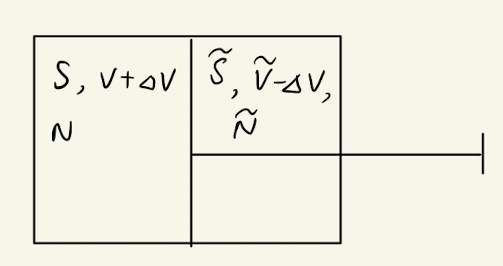
\includegraphics[width=0.8\textwidth]{images/0702-01.png}
	\caption{Composite system}
\end{figure}

Using the additivity postulate:
\begin{equation}
	\Delta U = U(S,V + \Delta V, N) + \tilde U (\tilde S, \tilde V - \Delta , \tilde N) -  (U(S,V,N)+U(\tilde S, \tilde V, \tilde N)) \geq 0
\end{equation}
The second term is the equilibrium energy, and it's minimised.

\textbf{Specialise to identical systems:}
\[ \tilde U = U \]
Then
\[ \Delta U = U(S,V+\Delta V, N )v+ U(S,V-\Delta V,N)-2U(S,V,N) \geq 0 \] 
For $ \Delta V  $ infinitesimal:
\[ \frac{\partial ^2 U}{\partial V^2} (\Delta V)^2 \] 
\[\implies \left( \frac{\partial ^2U}{\partial V^2} \right)_{S,N} \geq 0 \]
\[ dU = TdS -PdV +\mu dN\] 
\[ \frac{\partial U}{\partial V}_{S,V} = -P \] 
\[ \left( \frac{\partial ^2U}{\partial ^2} \right)_{S,N} = - \frac{1}{ \left ( \frac{\partial V}{\partial P} \right)_{S,V} } \] 
\[ = \frac{1}{V K_s} \geq 0 \] 
\begin{equation}
	K_s > 0
\end{equation}
where $ K_s $ is the isentropic compressibility. 

\subsection{Heat Transfer}
\[ \Delta U = U(S + \Delta S,V, N )v+ U(S - \Delta S,V,N)-2U(S,V,N) \geq 0 \] 
\[ \left (\frac{\partial ^2U}{\partial S^2} \right )_{V,N} \geq 0 \] 
\[ \left (\frac{\partial U}{\partial S} \right )_{V,N} = T \implies \] 
\[ \left (\frac{\partial ^2U}{\partial S^2} \right )_{V,N} = \left (\frac{\partial T}{\partial S} \right )_{V,N} = \left[ \left (\frac{\partial S}{\partial T} \right )_{V,N} \right]^{-1} ] \] 
\[ = \left[\frac{N}{T} \frac{T}{N}\left (\frac{\partial S}{\partial T} \right )_{V,N} \right ]^{-1} \geq 0\] 

\subsection{Volume Exchange for Helmholtz Free Energy}
\[ \Delta F = F(T,V+\Delta V, N) + F(T,V-\Delta V, N) -2F(T,V,N) \geq 0 \] 
\[ \left (\frac{\partial ^2F}{\partial V^2} \right )_{T,N} \geq 0  \] 
\[ \implies \left (\frac{\partial F}{\partial V} \right )_{T,N} = -P \] 
\[ \left (\frac{\partial ^2F}{\partial V^2} \right )_{T,N} = \left (\frac{\partial P}{\partial V} \right )_{T,N} = \left[ v \frac{1}{-v} \left (\frac{\partial V}{\partial P} \right )_{T,N} \right]^{-1}  \] 
\[ \frac{1}{VK_T} \geq 0 \] 
\[ \implies K_T \geq 0 \] 

\subsection{Heat Exchange for Enthalpy}
\[ H(S+\Delta S, P,N) + H(S-\Delta S, P,N) - 2H(S,P,N) \geq 0 \] 
\[ \implies \left (\frac{\partial ^2H}{\partial S^2} \right )_{P,N} \geq 0 \] 
\[ \left (\frac{\partial H}{\partial S} \right )_{P,N} = T \] 
\[ \left (\frac{\partial ^2H}{\partial S^2} \right )_{P,N} = \left[ \left (\frac{\partial S}{\partial T} \right )_{P,N} \right]^{-1} \geq 0 \] 
\[ \implies C_p \geq 0 \] 
\begin{shaded*}
	The stability conditions that we have derived so far are only valid for \textbf{extensive} variables!
\end{shaded*}
\subsection{What about intensive variables?}
We use TD relations.
\[ \left (\frac{\partial F}{\partial T} \right )_{V,N} = -S, \quad \left (\frac{\partial ^2F}{\partial T^2} \right )_{V,N} = - \left (\frac{\partial S}{\partial T} \right ) = \frac{-1}{\left (\frac{\partial ^2U}{\partial S^2} \right )_{V,N}} < 0\]
\[ \left (\frac{\partial U}{\partial S} \right )_{V,N} = T, \quad \left (\frac{\partial ^2U}{\partial S^2} \right )_{V,N} \] 
so
\begin{equation}
	\left (\frac{\partial ^2F}{\partial T^2} \right )_{V,N} < 0
\end{equation}

\subsection{Van der Waal's gas}
Ideal gas: \[ F = - Nk_bT\left[ ln (\frac{V}{N}) + \frac{3}{2}ln(k_BT) +X \right]  \] 
\textbf{Free, non-interacting particles} \\
Include interactions "treated crudely": \\

\begin{figure}[h]
	\centering
	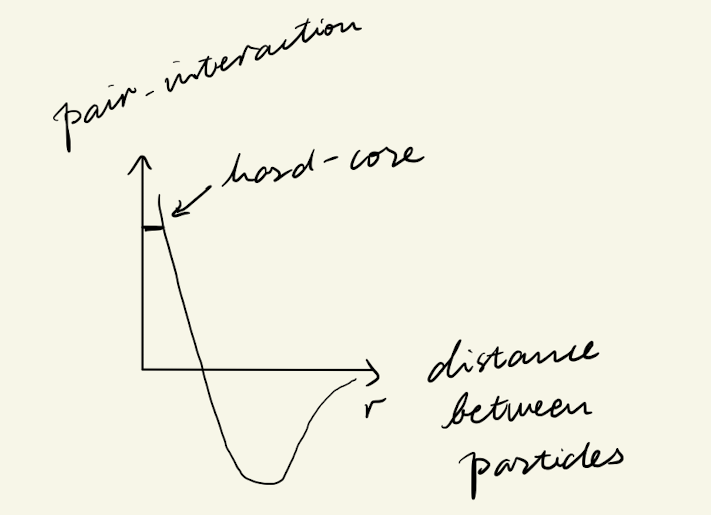
\includegraphics[width=0.8\textwidth]{images/0702-02.png}
	\caption{Van der Waal interaction model.}
	\label{fig:VDW}
\end{figure}
The interaction has two main effects:
\begin{enumerate}
	\item Energy is lowered by the mean interaction energy $ \propto \frac{N}{V}$ per particle.
	\item The hard-core potential restricts the volume to $ V \to V-Nb $ 
\end{enumerate}
\[ F_{VDW} = - Nk_BT \left[ ln(\frac{V-Nb}{N}) + \frac{3}{2} ln(k_BT) + X \right]  - a \frac{N^2}{V}\] 
where $ a $ (measure of attraction) and $ b $ (hard-core) are constants.
This is an extensive system, meaning we could use the Euler's equation. \\
\textbf{Pressure:} 
\[ P = - \left (\frac{\partial F}{\partial V} \right )_{T,N} =  \frac{Nk_BT}{V-Nb} + a \frac{N^2}{V^2} \] 

\begin{figure}[h]
	\centering
	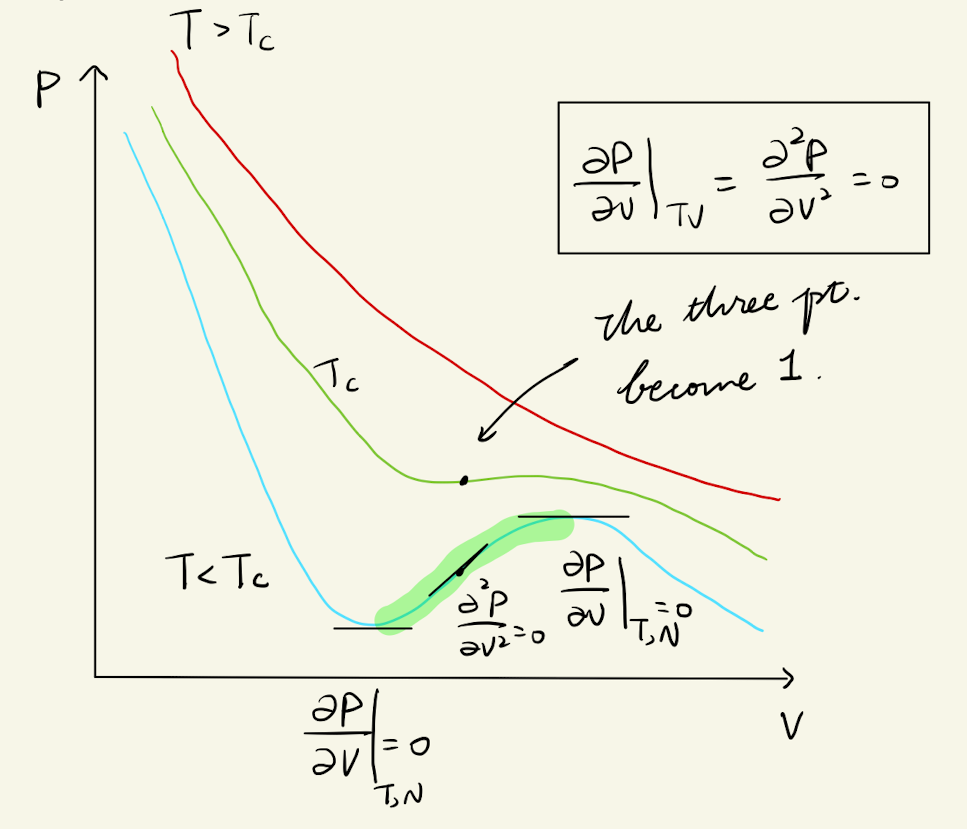
\includegraphics[width=0.8\textwidth]{images/0702-03.png}
	\caption{Pressure vs Volume diagram.}
	\label{fig:PvsV}
\end{figure}
\textbf{Stability:} 
\[ \left (\frac{\partial ^2F}{\partial V^2} \right )_{T,N} \geq \] 
\[ \left (\frac{\partial F}{\partial V} \right )_{T,N} = -P \] 
\[ \left (\frac{\partial ^2F}{\partial V^2} \right )_{T,N} = - \left (\frac{\partial P}{\partial V} \right )_T,N) > 0 \] 
\[ \implies  \left (\frac{\partial P}{\partial V} \right )_{T,N} < 0\] 
The highlighted part is unstable since $ \left (\frac{\partial P}{\partial V} \right )_{T,N} \geq 0 $.  \\

Want to calculate the critical temperature $ T_c $:

\[ \left (\frac{\partial P}{\partial V} \right )_{T,N} = 0 = \left (\frac{\partial ^2P}{\partial V^2} \right )_{T,N} = 0 \] 
\[ \frac{\partial P}{\partial V} = \frac{-Nk_BT}{(V_Nb)^2} + 2a \frac{N^2}{V^3} = 0\] 
\[ \implies Nk_BTV^3 = 2aN^2 (V-Nb)^2 \] 
\[  (\frac{\partial ^2P}{\partial V^2}   = \frac{2Nk_BT}{(V-Nb)^3} - 6a \frac{N^2}{V^{4}} = 0\] 
\[ \implies 2Nk_BTV^4 = 6aN^2(V-Nb)^3 \] 
Combine:
\[ 2V = 3(V-Nb) \] 
\begin{shaded*}
	\[ \implies V_c = 3Nb \] 
and
\[ k_BT_c = \frac{2aN^2(3Nb-Nb)^2}{N(3Nb)^3} =  \frac{8}{27}\frac{a}{b}\] 
\[ P_c = \frac{N_kBT}{V_c-Nb} - a \frac{N^2}{V_c^2} = \frac{1}{27}\frac{a}{b^2} \] 
\[ \frac{P_cV_c}{Nk_BT_c} = \frac{3}{8} \] Ideal gas: 1
\end{shaded*}

\textbf{insert Fig.4} 
Both unphysical, unstable.
\[ P = -\left (\frac{\partial F}{\partial V} \right )_{T.N} \] 
\[ \left (\frac{\partial P}{\partial V} \right )_{T,N} = - \left (\frac{\partial ^2F}{\partial V^2} \right )_{T,N} < 0 \] 
For stability.
\[ V = \left (\frac{\partial G}{\partial P} \right )_{T,N}\] 
\[ \left (\frac{\partial V}{\partial P} \right )_{T,N} = \left (\frac{\partial ^2G}{\partial P^2} \right )_{T,N} < 0 \] second derivative of intensive variabel less than $ 0 $ for stability. 

\textbf{insert Fig.5} 
Cap:Van der Waal's gas at $ T < T_C $ 
Stability
\[ \left (\frac{\partial ^2F}{\partial V^2} \right )_{T,N} > 0 \Rightarrow \left (\frac{\partial P}{\partial V} \right )_{T,N} < 0\] 
This is violated on D-F. Assumption of homogeneity breaks down. The homogeneous solution is unstable (unphysical. NOT realised) on D-F.

\textbf{insert Fig.6}
Maxwell construct: Choose a line which crosses the graph 3 times which also divides the area into $ 2 $ equal parts.
In the region B-H there are 3 possible values for $ V $ given a $ P $ (one is unphysical (DF), but there are still two to choose from.)
TD stable state at const. $ P,T,N $ minimises \textbf{Gibbs free energy}. 
Calculate $ G $ !
Van der Waal's gas is extensive: \[ U = TS - PV + \mu N \] 
\[ G = U - TS + PV = \mu N \] 
Recall Gibbs-Duhem relation: \[ d\mu = - \left(\frac{S}{N} \right)dT + \left( \frac{V}{N} \right) dP = \frac{V}{N}dP \] 
\[ \implies G = \int dG = \int d \mu N  = \int dP V\] Area under the curve.


\[ V = \left (\frac{\partial G}{\partial P} \right )_{T,N} \] 
At $ C,G $ there are two phases that coexists: $ V_C $ and $ V_G $
Since $ V_C $ is bigger than $ V_G $, so $ V_C $ describes a gas phase and $ V_C $ describes a liquid phase.

\textbf{insert Fig.8 and 9} 
\[ \rho _C = \frac{N}{V_C}, \quad \rho_G = \frac{N}{V_G} \] 

\subsection{Phases}
C-phase: $ V_C $ volume fraction $ \frac{V_C}{V} = X_C $ 
G-phase: $ V_G $ volume fraction $ \frac{V_G}{V} = X_G $ 
\[ \implies V_C + V_G = V \implies X_C + X_G = 1 \] 
Total number of particles:
\[ N = V_C \rho_C^{*} + V_G \rho_G^{*} \] 
\[ \frac{N}{V} = X_C \rho_{C}^{*} + X_G \rho_{G}^{*}   \] 
Set $ X_G = 1 - X_C, $ $ \frac{N}{V} $ 
\[ \rho = X_C \rho_C^{*} + (1-X_C) \rho_{G}^{*}  \] 
\[ X_C = \frac{\rho - \rho_{G}^{*} }{\rho_{C}^{*} - \rho_{G}^{*} }, \quad X_G = 1 - X_C\] 

\textbf{insert Fig.10} 
From Helmholtz Free energy, $ T < T_C $ 

\textbf{insert Fig.11} 
\[ P = - \left (\frac{\partial F}{\partial V} \right )_{T,N} \] 

\textbf{insert Fig.12} 
\subsection{Clausius-Clapeyron}
Assume extensivity $ \implies $ Gibbs-Duhem relation
\[ d\mu = -\frac{S}{N}dT + \frac{V}{N}dP = -sdT + \frac{1}{n}dP \] 
where $ s \equiv \frac{S}{N}, \quad n \equiv \frac{N}{V} $ 

Liquid
\[ \mu_2^{l} - \mu_1^{l} = -s(T_2^{l}-T_1^{l}) + \frac{1}{n^{l}}(P_2^{l}-P_1^{l})\] 
Gas
\[ \mu_2^{l} - \mu_1^{l} = -s(T_2^{l}-T_1^{l}) + \frac{1}{n^{l}}(P_2^{l}-P_1^{l})\] 
$ l $ stands for liquid
On the ceexistence line in equilibrium:
\[ \mu_1^{l} = \mu_1^{g} \] same with all other variables.
Subtract the eqs:
\[ 0 = (s^{g}-s^{l})(T_2 - T_1) + \left( \frac{1}{n^{l}} - \frac{1}{n^{g}} \right)(P_2-P_1)  \] 
\[ \implies \frac{P_2-P_1}{T_2-T_1} = \frac{s^{g} - s^{l}}{T_2-T_1} = \frac{s^{g}-s^{l}}{\frac{1}{n^{g}} - \frac{1}{n^{l}}} \] 
\[ \implies \left (\frac{\partial P}{\partial T} \right )_{\text{alone coexistence}} = \frac{(s^{g}-s^{l})}{ \frac{1}{n^{g}} - \frac{1}{n^{l}}}\] 


\section{More particle types: Gibbs Phase Rule}
\[ dU = TdS -PdV + \sum_{i=1}^{K} \mu_i dN_i\] 
There are $ 2+K $ independent variable.
Extensive:
\[ U = TS-PV+\sum_{i=1}^{k} \mu_i N_i \] 
Gibbs-Duhem:
\[ d\mu = -\frac{S}{N} dT + \frac{V}{N}dP + \sum_{i=1}^{k}N_i d\mu_i \] 
If we have $ \phi $ phases, then there is a Gibbs-Duhem rel. for each phase.
\[ 0 = S^{1} dT^{1} -V^{1}dP^{1} + \sum_{i=1}^{k}N_i^{1}d\mu_i^{1}\] phase 1
\[ \vdots \] 
\[ 0 = S^{\phi} dT^{\phi} -V{\phi}dP^{\phi} + \sum_{i=\phi}^{k}N_i^{\phi}d\mu_i^{\phi}\] phase $ \phi $ \\
\textbf{At coexistence:} 
\[ T_1=T_2=...=T_\phi \quad P_1=P_2=...=P_\phi \quad \forall i \mu_i^{1} = \mu_i^{2} = ... =\mu_i^{\phi}\] 
(Can omit superscript from T,P, and $ \mu_i $ )

\[ 0 = S^{1}dT - V^{1}dP + \sum_{i=1}^{k} N_i^{1} d\mu_i \] 
and for all $ \phi $ equations.
There are $ 2+k $ variables $(T,P,\mu_i)$ and $ \phi $ equations.
The number of \textbf{free variables} at coexistence determines the dimension of the coexistence manifold (multidimensional object).
\[ F = 2+K-\phi \]

\begin{example}[K=1]
	\[ F = 3 - \phi \] 
	$ \phi=2 $ (Two phases coexist) $\implies F=1$ (line)
	$ \phi=3 $ (Three phases coexist) $\implies  F=0 $ (point)
	$ \phi=4 $ cannot coexist.  
\end{example}

\begin{example}[Binary Alloy (Two types of atoms)] 
	\[ K=2 \] 
	\[ F = 4 - \phi \] 
	Here $ 4 $ phases can coexist at a point, $ 3 $ along a line and $ 2 $ on a surface.
\end{example}

\section{3. Law of TD}
``The entropy of a (real QM) TD system goes to a constant as $ T \to 0 $. ''\\
Violated for the ideal gas:
\[ S = k_BN (\frac{3}{2}ln\left( \frac{U}{N} \right) + ln\left( \frac{V}{N} \right) ) + X \] 
\[ = k_B N\left(\frac{3}{2} ln \left(\frac{3}{2} \frac{Nk_BT}{N} \right) + ln\left( \frac{V}{N} \right) +X \right) \] 
when $ T \to 0 $, $ S \to -\infty $  

Planck said it's $ 0 $, but it's \textbf{NOT}! 
\subsection{Consequences}
\[ dS = \frac{ \text{\dj}Q }{T} \quad \text{\dj}Q = cdT\]
\[ dS = c \frac{dT}{T}, S(T)-S(0) = \int_0^{T}dS = \int_0^{T} \frac{dT}{T} C \] 
Taking $ T \to 0 $ will give $ 0 $ if integral is not diverging. For integral not to diverge $ C(T \to 0) = 0 $ \\

Also the thermal expansion coefficient:
\[ \alpha = \frac{1}{V}\left( \frac{\partial V}{\partial T} \right)_{P,N} = -\frac{1}{V} \left( \frac{\partial S}{\partial P} \right)_{T,N} \] 
\[ -SdT + V dP. \] 
If $ S $ goes to a pressure independent const. at $ T \to 0 $. Then $ \alpha=0 $.


\newpage
\chapter{Statistical Mechanics}
\section{Behaviour for Large N}
\subsection{Binomial Distribution}
Probability distribution for flipping coins:
1 coin: \[ 1:1 \] 
2 coins: \[ 1:2:1 \] 
3 coins: \[ 1:3:3:1 \] 

Mean value, increases width increases, maximum (probability) decreases.
\[ P(N_{\uparrow}) = \frac{1}{2}^{\uparrow} \frac{1}{2}^{\downarrow} = \frac{N!}{N^{\uparrow}! (N-N^{\uparrow})!} \frac{1}{2}^{N}\] 
What is the characteristic of this distribution when $ N $ is large. We need $ N! $ for $ N $ large
\[ N! = \int_0^{\infty} dx \: x^{N} e^{-x} = \left( -x^{N}e^{-x} |_0^{\infty} + N \int_0^{\infty} dx x^{N-1}e^{-x} \quad \text{and so on}\right) \] 
\textbf{Factorial Expansion} 
\begin{equation}
	N! = \int_0^{\infty} dx e^{-x+Nln(X)}
\end{equation}
Use Laplace's method. For $ N $ large Approximate the integrand by its value close to the maximum of the exponent.
Set \[ g(x) = Nln(x)-x \] 
\[ \left( \frac{\partial g}{\partial x} \right) = \frac{N}{x}-1 = 0  \implies X_0 = N\] 
\[ 2\left( \frac{\partial g}{\partial x} \right) = -\frac{N}{x^2} |_{x=x_0} = -\frac{1}{N} < 0 \implies x_0 \text{is a max.}   \] 
\[ g(x) \approx g(x_0) + \left( \frac{\partial g}{\partial x} \right)_{x_0}(x-x_0) + \frac{1}{2} 2\left( \frac{\partial g}{\partial x} \right)_{x=x_0}(x-x_0)^2   \] 
\[ \implies N! = \int_{{0}}^{{\infty}} {dx} {e^{Nln(N)-N- \frac{1}{2N} (x-N)^2}} \] 
\[ = e^{Nln(N)-N} \int_0^{\infty} e^{- \frac{1}{2N}(x-N)^2} \] 
For $ N >> \sqrt(N) \text{width of the Gaussian} $ we can extend the lower limit to $ -\infty $ since it's so small.
\[ \implies e^{Nln(N)-N} \int_{-\infty}^{\infty} dx e^{- \frac{1}{2N}x^2} \] 
\[ = e^{Nln(N)-N} \sqrt{2\pi N} \] 

\begin{shaded*}	
	\textbf{Stirling Approximation} 
\begin{equation}
	ln(N!) = Nln(N)-N + \frac{1}{2}ln(2\pi N)
\end{equation}
The last term is often dropped when $ N >> \sqrt{N} $ 
\end{shaded*}

\[ ln(P(N_{\uparrow})) = ln(N_{\downarrow}) - ln(N_{\uparrow}) - ln\left( (N-N_{\uparrow})! \right)+ N_{\uparrow}ln(P) + (N - N_{\uparrow})ln(1-p) \] 
\[ = Nln(N) - N  - (N_\uparrow ln(N_{\uparrow}) - N_\uparrow) - \left( (N-N_\uparrow) ln(N-N_\uparrow) - (N-N_\uparrow) \right) + N_\uparrow ln(P) + (N -N_{\uparrow}) ln(1-P)\] 
\[ = Nln(N) -N_{\uparrow} ln(N_\uparrow) - (N-N_\uparrow)ln(N-N_\uparrow) + N_\uparrow ln (\frac{P}{1-p}) + Nln(1-P)\] 

\textbf{Maximum:} 
\[ \left( \frac{\partial }{\partial N_\uparrow} \right) ln[P(N_\uparrow)] \implies 
- ln(N_\uparrow)- \frac{N_\uparrow}{N_\uparrow} + ln(N-N_\uparrow) + 1 + ln(\frac{p}{1-p}) = 0\] 

\[ \implies ln(\frac{p}{1-p}) = ln(\frac{N_\uparrow}{N-N_\uparrow}) = ln\left( \frac{N_\uparrow/N}{1 - N_\uparrow /N} \right) \] 
\[ \implies P = \frac{N_\uparrow}{N} \] 
\[ \implies N_\uparrow^{max} = NP \] 
\textbf{Location of the max $P$ is $ NP $. } 
Second derivative:
\[ \left( \frac{\partial^2 ln(P)}{\partial N_\uparrow^2} \right)  = -\frac{1}{N_\uparrow} - \frac{1}{N-N_\uparrow}\] 
\[ = -\frac{1}{N}(\frac{1}{N_\uparrow/N} + \frac{1}{1-N_\uparrow/N}) = -\frac{1}{N}\left( \frac{1}{(N_\uparrow/N)(1-N_\uparrow/N)} \right) \] 
\[ =^{at max \frac{N_\uparrow}{N} = p} = -\frac{1}{N}\frac{1}{p(1-p)}\] 

\[ ln(P_N)|_{\text{at max}} = NlnN -Np(lnN+lnP) -N(1-p)(ln(N)+ln(1-P)) + NPln(1-p) + Nln(1-p) = 0\] 

\[ ln[P(N_\uparrow)]  = 0 + \underbrace{0}_{\text{first der.}} - \frac{1}{2(Np(1-P))} (N_\uparrow - NP)^2\] 
\[ P(N_\uparrow) \approx {\color{red} A } e^{-\frac{1}{2N(1-p)}(N_\uparrow-NP)^2} \] 
where {\color{red} A} is the missing normalisation constant. \\
\textbf{Gaussian around $ NP \propto N $ and standard derivative $ \sqrt{NP(1-P)} \propto \sqrt{N} $ } \\
The height is $ \frac{1}{\sqrt{N}} $. \\
If we focus on the fraction of coins being head,
\[ \left \langle \frac{N_\uparrow}{N} \rangle \right> = p\] 
\[ \left \langle \left(  \frac{N_\uparrow}{N}^2 \right ) \right \rangle - \left \langle \frac{N_\uparrow}{N} \right \rangle^2 = \frac{1}{N^2} NP(1-P) \propto \frac{1}{N}\] 
the mean value becomes a precise statment as $ N \to \infty $ 
\subsection{Random Independent Variables}
We define a random variable $ F $ that takes $ 2 $ values \\
1 with Probability $ P $ 
0 with probability $ 1-P $ 
Then take $ N $ such random variables $ F_i \quad i = 1 \cdots N $ then
\[ N_\uparrow = \sum_{i=1}^{N} F_i \] 
The average value of $ F_i $ is 
\[ \left \langle F_i \rangle \right> = 1P + 0(1-P)  = P\] 
	\[ \left \langle N_\uparrow \right \rangle = \left \langle \sum_{i=1}^{N}F_i \right \rangle= \sum_{i=1}^{N} \left \langle F_i \right \rangle = NP\] 
Deviation from the average:
\[ \left \langle (N_\uparrow -NP)^2 \right \rangle = \left \langle N_\uparrow^2 \right \rangle - 2NP \left \langle N_\uparrow \right \rangle + (NP)^2\]
		\[ \left \langle N_\uparrow^2 \right \rangle= \left \langle \left( \sum_{i=1}^{N} F_i \right)^2  \right \rangle= \left \langle \sum_{i=1}^{N}F_i \sum_{j=1}^{{N}} F_j\right \rangle = \left \langle \sum_{n=0}^{N} F_i^2 + \sum_{i,j} F_i F_j\right \rangle\] 
\[ = \sum_{i=1}^{N} \left \langle F_i^2 \right \rangle + \sum_{i\neq j} \left \langle F_i F_j \right \rangle \] 
\[ = \frac{1}{N^2}NP(1-P) \] 

\section{Boltzmann Configurational Entropy}

\begin{figure}[htpb]
\begin{center}
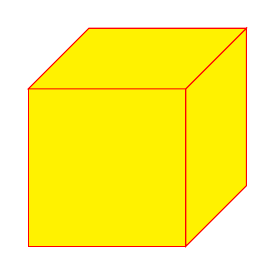
\begin{tikzpicture}[scale=1, transform shape]
	\pgfmathsetmacro{\cubex}{2}
\pgfmathsetmacro{\cubey}{2}
\pgfmathsetmacro{\cubez}{2}
\draw[red,fill=yellow] (0,0,0) -- ++(-\cubex,0,0) -- ++(0,-\cubey,0) -- ++(\cubex,0,0) -- cycle;
\draw[red,fill=yellow] (0,0,0) -- ++(0,0,-\cubez) -- ++(0,-\cubey,0) -- ++(0,0,\cubez) -- cycle;
\draw[red,fill=yellow] (0,0,0) -- ++(-\cubex,0,0) -- ++(0,0,-\cubez) -- ++(\cubex,0,0) -- cycle;
\end{tikzpicture}
\end{center}
\caption{A 3D box with $ V = L^3 $ with $ N $ identical particles, labelled by their $ x $-cordinates }%
\label{fig:box}
\end{figure}
"The number of microstates $ \propto L^3$ "\\
Since $ x_1 $ has to be in the left of $ x_2 $ and same for the other particles:
\[ \text{\# of microstates}  = \int_0^{L} dx_N L^2 \cdots \int_{0}^{x_3} dx_2 L^2 \int_{0}^{x_2} dx_1 L^2 \] 
\[ = L^{2N} \int_{0}^{L} dx_N \int_{0}^{x_N} dx_{N-1}  ... \int_0^{x_3}dx^2 \int_{0}^{x_2}dx_1  \] 
Integrating from the right hand side we see a pattern: 
\[ x_2 \rightarrow \frac{x_3^2}{2!} \rightarrow \frac{x_4^3}{3!} \cdots \] 
\[ = L^{2N} \frac{L^{N}}{N!} = \frac{V^{N}}{N!} \] 
This is the same result as gotten with first labelling particles and then divide by all permutations of labels.

\begin{figure}[htpb]
\begin{center}
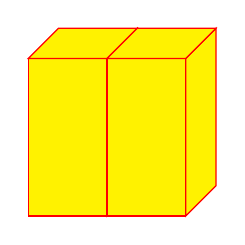
\begin{tikzpicture}[scale=1, transform shape]
\pgfmathsetmacro{\cubex}{1}
\pgfmathsetmacro{\cubey}{2}
\pgfmathsetmacro{\cubez}{1}
\draw[red,fill=yellow] (0,0,0) -- ++(-\cubex,0,0) -- ++(0,-\cubey,0) -- ++(\cubex,0,0) -- cycle;
\draw[red,fill=yellow] (0,0,0) -- ++(0,0,-\cubez) -- ++(0,-\cubey,0) -- ++(0,0,\cubez) -- cycle;
\draw[red,fill=yellow] (0,0,0) -- ++(-\cubex,0,0) -- ++(0,0,-\cubez) -- ++(\cubex,0,0) -- cycle;
\pgfmathsetmacro{\cubex}{1}
\pgfmathsetmacro{\cubey}{2}
\pgfmathsetmacro{\cubez}{1}
\draw[red,fill=yellow] (1,0,0) -- ++(-\cubex,0,0) -- ++(0,-\cubey,0) -- ++(\cubex,0,0) -- cycle;
\draw[red,fill=yellow] (1,0,0) -- ++(0,0,-\cubez) -- ++(0,-\cubey,0) -- ++(0,0,\cubez) -- cycle;
\draw[red,fill=yellow] (1,0,0) -- ++(-\cubex,0,0) -- ++(0,0,-\cubez) -- ++(\cubex,0,0) -- cycle;
\end{tikzpicture}
\end{center}
\caption{2 boxes.}%
\label{fig:}
\end{figure}

Assuming all the microstates are equally probable.
\[ P(N_A, N_B) = \frac{ \frac{V_A^{N_A}}{N_A!} \frac{V_B^{N_B}}{N_B!} } {\frac{V^{N}}{N!}}\] 
\[ = \frac{N!}{N_A!N_B!} \left( \frac{V_A}{V} \right) ^{N_A} \left( \frac{V_B}{N_B} \right)^{N_B}  \] 
(Binomial distribution)
Boltzmann: All microstates (position here) are equally likely. The most likely macrostate (value of $ N_A, N_B $ is the one that corresponds to most microstates: i.e. the max of $P(N_A, N_B))$. \\

The maximum of $ P(N_A,N_B) $ also corresponds to the maximum of
\begin{equation}
	\label{eq:bce}
	 k_Bln\left( P(N_A,N_B) \frac{V^N}{N!} e^{XN} \right)  
 \end{equation}
\textbf{ $ S_B $ Boltzmann Configuration Entropy } 
Boltzmann never actually wrote this.

Equation~\ref{eq:bce} can also be written as
\[ kln((\frac{V_A^{N_A}}{N_A!}) e^{xN_A} \frac{V_B^{N_B}}{N_B!} e^{xN_B}) \] 

\textbf{\textit{The other words, the impossibility of an uncompensated decrease of entropy seems to be reduced to an improbability. (Boltzmann,1898)}}

Set $ \Omega \equiv \frac{V^{N}}{N!} $ 
In equilibrium:
\[ S_B = \underbrace{kln(P_{max} \Omega e^{xN})}_{klnP_{max}+kln(\Omega e^{xN})} = kln( \Omega_A  e^{xN_A}) + kln(\Omega_B e^{xN_B})\] 

\[ LHS = kln(\Omega e^{XN}), \]
Note that this has the same form as the right hand side! \\
So in the TD equilibrium,
\begin{equation}
	S = kln(\Omega e^{XN}) = kln(\Omega) + kXN
\end{equation}
This is additive  over its subsystems.
\[ S = S_A + S_B \] 
\begin{equation}
	\Omega = \frac{V^{N}}{N!} = \frac{ \int d^3 q_1 \cdots \int d^3 q_n }{N!}
\end{equation}

To generalise to also include momenta and pick only those configurations that have a total energy $ E $.

\[ \Omega(E) \delta E \] $ \delta E $ is a thin energy shell
\[ \frac{1}{N! h^{3N}}= \int d^q 1_1 \cdots \int d_3 q_N \int d^p 1_1 \cdots  \int d^3 p_N\] 
the $ h^{3N} $ can be interpreted as the $ x $ from before, the reference volume phase space.It's a related to the uncertainty, and it's a choice.

\begin{remark}
	\[ ln(h^{3N}) = Nln(h^{3}) \] 
\end{remark}

\begin{equation}
	\Omega(E)\delta E = \frac{1}{N!h^{3^{N}}} \int d^3 q_1 \cdots d^3 p_N (\Theta(E+\delta E -H(q_1, \cdots, p_N) ) -\Theta (E-H(q_1 \cdots p_N))) 
\end{equation}
where the $ \Theta (x) $ is the Heaviside step function.
Expand for small $ \delta E $ 
\[ = \delta E \frac{1}{N!h^{3N}} \int d^3 q_1 \cdots d^3 p_N \delta (E- H(q_1 \cdots p_N)) \] 

\begin{shaded*}
\begin{equation}
	\Omega(E) = \frac{1}{N!h^{3N}} \int d^3 q_1 \cdots d^3 p_N \delta (E- H(q_1 \cdots p_N)) 
\end{equation}
\textbf{This is the microcanonical ensemble. (All microstates have the same energy.)} 
\end{shaded*}

\section{Equilibrium Stat Mech and Ensembles}
After a time the system reaches equilibrium (when the macroscopic states is time independent and is independant of the initial condition.)
Microscopic state changes all the time (also in equilibrium) \\
Microscopic state: 
$$ Q = \{q_{1x}, q_{1y}, q_{1z}, ... q_{Nz}\} $$
\[ P = \{p_{1x}, p_{1y} ...\}\] 
$ \{Q,P\} $ has 6N components.
A microstate is a point in phase-space.
\subsection{Conserved Quantities}
In the approach to equilibrium, not all info about the initial state is lost. If collisions conserves energy, then (total) energy is conserved. \\
Instead of considering the microstates at different times, evolving from a particular initial condition, we can consider the system at a particular time $ t $, coming from all possible initial conditions with the same energy.

\[ \Omega(E) = \frac{1}{N!h^{3N}} \int D\mathbb{Q} D\mathbb{P} \delta(E - H(\mathbb{P} - \mathbb{Q}))\] 
\begin{equation}
	S = k_B ln(\Omega(E)\delta E)
\end{equation}

\textbf{Ensemble average}

\[ \left \langle   O \right \rangle_E = \frac{1}{\Omega(E)} \frac{1}{N!h^{3N}}\int D\mathbb{P} D \mathbb{Q} \delta(E-H(\mathbb{P},\mathbb{Q}))O(\mathbb{P},\mathbb{Q})\] 
\pagebreak
\section{Microcanoical Ensemble}
Ideal gas and Maxwell-Boltzmann distribution.
Microcanonical ensemble:
\[ S = k_B ln(\Omega) \] 
\[ \Omega = \Omega(E) \delta E  = \int \frac{1}{N!h^{3N}} \int d^3 q_1 \cdots d^3 p_N \: \delta (E- H(\mathbb{P}, \mathbb{Q})) \delta E \] 
\textbf{Ideal Gas:} 
\[ H = \sum_{n=1}^{N} \frac{\vec{p_i}^2}{2m}\] 
All $ q $'s will be inside the box of volume $ V $.

First the integrals over $ q $'s give $ V^{N} $ (They are independant of the positions, but need to be confined in the box.)
\[ \Omega = \frac{V^{N}}{N!h^{3N}} \delta E \int d^3p_1 \cdots d^3 p_N \: \delta (E - \sum_{i=1}^{N} \frac{\vec{p_i}^2}{2m}) \equiv \frac{V^{N}}{N! h^{3N}} \delta E \] 
Note that it's possible to take any momentum. \\
Shift:
\[ \vec{p_i}\prime = \frac{\vec{p_i}}{\sqrt{2m}} \]
\[(2m)^{\frac{3N}{2}} \int d^3p_1 \prime \cdots d^3p_N \prime \delta (E - \sum_{i=1}^{N} \underbrace{\vec{p_i}^2)}_{3N terms}\] 
Expanding these out and call them $ r^2 $
\[ r^2 = p_1^{{x}^2} + p_1^{{y}^2} + p_1^{{z}^2} + ... + p_N^{{z}^2} \] 
\begin{shaded*}
Switch to hyperspherical coordinates in $ 3N $ dimensions.
\[ I = (2m)^{\frac{3N}{2}} \int d \tilde \Omega^{3N-1} \int_0^{\infty} dr V^{3N-1} \delta (E-r^2)\] 
\end{shaded*}

Now use \[ \int dx f(x) \delta(g(x)) = \sum_{n} \frac{f(x)}{|g \prime (x)|} |_{x=x_n}\] 
\begin{equation}
	\label{eq:int-dr}
	\int dr \: r^{3N-1} \delta (E - r^2)
\end{equation} 
\[ |g \prime (r)| = |-2r| = 2r \] 
\textbf{Zeros of g: $ r = \pm \sqrt{E} $ } but only $ +\sqrt{E} $ is indside the integration range. \\
Then
\[ \int dr \: r^{3N-1} \delta (E - r^2) = \frac{E^{\frac{3N-1}{2}}}{2E^{1/2}} = \frac{E^{\frac{3N}{2}}}{2}\] 
So
\[ I = (2m)^{\frac{3N}{2}} \tilde \Omega^{3N-1} (2m)^{3N/2} \frac{E^{\frac{3N}{2}-1}}{2} \] 

For the \textbf{Solid Angle} $ \tilde \Omega^{d-1} $ in $ d $ dimensions 
We consider a Gaussian Integral and compute it in both hyperspherical and Cartesian coordinates.
\[ I = \int d^{d} r e^{-r^2} = \int d \tilde \Omega^{d-1} \int_0^{\infty} r^{d-1} e^{-r^2} \] 
Change variables:
\[ t = r^2 \quad dt = 2r dr \]
\[ I = \frac{1}{2} \: \tilde \Omega^{d-1} \underbrace{\int_0^{\infty} t^{\frac{d}{2}-1} e^{-t}}_{\Gamma(\frac{d}{2})}\]

Then in Cartesian coordinates:
\[ I = \int_0^{\infty} dx \cdots \int_{-\infty}^{\infty} e^{-x_1^2}e^{-x_2^2}\cdots e^{-x_d^{d}} = \pi^{\frac{d}{2}} \] 
\begin{shaded*}
\begin{equation}
	\tilde \Omega^{{d-1}} = \frac{2 \pi \frac{d}{2}}{\Gamma(d/2)}
\end{equation}
\end{shaded*}
\[ \Omega =  \frac{V^{N}}{N!h^{3N}} \delta E \tilde \Omega^{3N-1} (2m)^{\frac{3N}{2}} \frac{E^{\frac{3N}{2}-1}}{2} \] 
where
\[ \tilde \Omega^{3N-1} = \frac{2\pi^{\frac{3N}{2}}}{\Gamma{\frac{3N}{2}}}\] 
\[ \Omega = \frac{V^{N}}{N!h^{3N}} \frac{(2 \pi m E )^{\frac{3N}{2}}}{\Gamma(\frac{3N}{2})} \frac{dE}{E}\] 
Finally the entropy is
\[ S = k_B ln(\Omega) = k_B ln(\left[ \frac{V(2 \pi m E)^{3/2}}{h^{3}} \right]^{N} \frac{dE}{N!\Gamma(3N/2)E} ) \] 
Now use \[ X \Gamma(x) = \Gamma(x+1) \implies \Gamma(3N/2) = \frac{2}{3N}\Gamma(\frac{3N}{2}+1) \] 
\[ S = k_B \left( ln\left[ \frac{V(2 \pi m E)^{3/2}}{h^{3}} \right]^{N} \right ) - k_B (NlnN-N) - k_B \left(\frac{3N}{2}ln \left(\frac{3N}{2}-\frac{3N}{2} \right) \right) - k_B ln \left(\frac{2E}{3N \delta E}\right)\] 
where we ignore the last term since it doesn't scale with $ n $.
\[ S = Nk_B \left[ ln \left(\frac{V}{N} \right) + \frac{3}{2} ln \left(\frac{E}{N} \right) + \frac{5}{2} + \frac{3}{2}ln\left( \frac{4\pi m}{3h^2} \right) \right ] \] 
\begin{shaded*}
The Sackur-Tetrode formular for entropy of ideal gas
\begin{equation}
	S = Nk_B \left( \frac{5}{2} - ln\left( \frac{N}{V} \underbrace{\left( \frac{h}{(\frac{4 \pi mE}{3N})^{\frac{1}{2}}} \right)^{\frac{1}{2}}}_{\lambda^{3}}  \right)^3  \right) 
\end{equation}
Expected to be valid physically when $ V >> N\lambda^3 $ 
\end{shaded*}

\pagebreak
\section{Maxwell-Boltmann Distribution}
\textbf{NOTATION: $ P \to $ Probability, $ p \to$ momentum  } \\
The probability of one particle having a momentum in one direction being of magnitude $ p_1 $ when the total energy is $ E $.
\[ P(p_1) = \frac{\text{Volume of phase-space where }p_{1x} = p_1 \text{ and the total energy is }E}{\text{Volume of phase-space with total energy} E}\] 
\[ = \frac{\text{The surface area of a sphere in }3N-1 \text{dimensions with radius} \sqrt{E-\frac{p_i^2}{2m}}}{\text{surface area of a sphere in }3N \text{dimensions with radius }\sqrt{E}} \] 
\[  = \frac{\pi ^{\frac{3N-1}{2}} (2m)^{\frac{3N-1}{2}} (E- \frac{p_i^2}{2m})^{(\frac{3N-1}{2}-1)} \Gamma(\frac{3N-1}{2})}{\pi ^{3N/2} (2m)^{3N/2} E^{3N/2 - 1} / \Gamma(3N/2)} \] 
\[ \frac{\Gamma{3N/2}\left(1-\frac{p^2}{2mE}\right)^{\frac{3N}{2}-\frac{3}{2}}}{\Gamma{\frac{3N-1}{2}}\sqrt{\pi}\sqrt{2mE}} \] 
In general $ \frac{p_i^2}{2mE} << 1 $
\[ 1 - \frac{p_i^2}{2mE} \not \approx e^{-\frac{p_i^2}{2mE}} \] 
\textbf{Stating the result without proof:} 
\[ \frac{\Gamma(3N/2)}{\Gamma(\frac{3N-1}{2})} \overbrace{\approx}^{N-large} \left (\frac{3N}{2} \right)^{ \frac{1}{2} } \]
To show this, use Stirling's formular and that the gamma function is factorial (somehow).

\[ P(p_1) = e^{\frac{-\frac{P^2}{2mE}(\frac{3N}{2} - \frac{3}{2})}{\sqrt{2 \pi m E}} \frac{3N}{2}^{ \frac{1}{2} }} \] 
\[  = \frac{1}{\sqrt{2 \pi \frac{2mE}{3N}}} e^{-\frac{p_i^2}{2\left( \frac{2mE}{3N} \right) }}\] 
Gaussian with mean $ 0 $, $ \sigma^2 = \frac{2mE}{3N} $. \\
For the ideal gas in TD:
\[ E = \frac{3}{2}Nk_bT \] 
\[ \sigma^2 = mk_BT \] 
We can in fact define the temperature in statistical mechanics as the width of the momentum distribution and use that definition to establish the equality: \[ E = \frac{3}{2}Nk_BT \] 

\section{Flow in Phase-space:Liouville theorem}
\textbf{Ensemble:} Several copies of the same system but with different initial conditions.
Insert phase space figure.
A point in the phase space is one system, an ensemble is many dots in the phase space. \\
Imagine so many copies of the system that on a course grained scale $ h_3N $, we can talk about a density of systems.
\[ \rho(q_1, \cdots, p_N, t) \] 
where $ \rho $ is the ensemble density. \\
So the number of systems in the region around $ q_1 ... p_N $  at time $ t $ is 
\[ \rho(\mathbb{Q}, \mathbb{P}, t) d\mathbb{Q} d\mathbb{P} \] 
when time goes on, the system will change (points in phase-space is moving) and so the ensemble density can in principle change. \\
Paths can't cross, but can merge, because from one point(initial condition) we can only have path. \\
Newton's equations are continuous, so a system(the trajectory, point) moves continuously in phase-space. This means that it does not disappear or reappear suddenly in phase space.
\subsection{Continuity Equation}
``in = out''
\[ \frac{\partial \rho}{\partial t}  = \vec{\nabla} \vec{j}  \] 
\[ \vec{j} = \rho \vec{V} \] where $ V $ is the generalised velocity. 
\[ \vec{V} = \left( \dot q_{1x} ... \dot p_{Nz} \right)  \] 
Continuity equation in terms of components:
\[ \frac{\partial \rho}{\partial t}  = \sum_{n=1}^{3N} \left( \frac{\partial (\rho \dot q_n)}{\partial q_n} + \frac{\partial (\rho \dot p_n)}{\partial p_n}  \right) \] 
\[ - \sum_{n=1}^{3N} \left( \left( \frac{\partial \rho}{\partial  q_n} \right) \dot q_n  + \frac{\partial \rho}{\partial p_n} \dot p_n + \rho \underbrace{\left( \frac{\partial \dot q_n}{\partial q_n} + \frac{\partial \dot p_n}{\partial p_n}  \right)}_{0} \right)  \] 

Hamilton eqs of motion:
\[ \dot q_n = \left( \frac{\partial H}{\partial p} \right) \implies \left( \frac{\partial \dot q_n}{\partial q_n} \right) -  \left( \frac{\partial^2 H}{\partial q_n \partial p_n} \right) \] 
using \[ \frac{\partial ^2J}{\partial q_n \partial p_n}  =  \frac{\partial ^2J}{\partial p_n \partial q_n} \] 

\paragraph{How does the density change as we flow with the system?}
\[ \frac{d}{dt} \: \rho(q_{1x}(t) \cdot p_{nz}(t), t) \]
\[ = \frac{\partial \rho}{\partial t} + \sum_{n=1}^{3N} \frac{\partial \rho}{\partial q_n} \dot q_n + \frac{\partial \rho}{\partial p_n} \dot p_n\] 
\[  = \frac{\partial \rho }{\partial t} - \frac{\partial \rho}{\partial t}   = 0\] 
No local change in density following a Volume element. \\
Flow in phase-space is as an incrompressible liquid (same volume different shape.) \\
\[ \frac{\partial \rho}{\partial t}  = -\sum_{n=1}^{3N} \left( \frac{\partial \rho}{\partial q_n} \frac{\partial H}{\partial p_n} - \frac{\partial \rho}{\partial p_n} \frac{\partial H}{\partial q_n} \right) = -\{\rho, H\} \] 

Recall $ \{\} $ is the Poisson bracket,
\[ \{A,B\} = \sum_{n=0}^{3N} \frac{\partial A}{\partial q_n} \frac{\partial B}{\partial p_n} - \frac{\partial A}{\partial p_n} \frac{\partial B}{\partial q_n}  \] 
which btw is the anticommutator in QM. \\

In equilibrium we want $ \frac{\partial \rho}{\partial t} = 0 $ 
\[ \{H, \rho\} = 0 \] 
Now note that is $ \rho = \rho(H) $ 
Then 
\[ \{H, \rho(H)\} = \sum_{n=1}^{3N} \left( \frac{\partial H}{\partial q_n} \frac{\partial \rho}{\partial H} \frac{\partial H}{\partial p_n} - \frac{\partial H}{\partial p_n} \frac{\partial \rho}{\partial H} \frac{\partial H}{\partial q_n} \right) = 0  \] 
That's the microcanonical ensemble (only depends on H)is constant in time.
\[ \rho(\mathbb{P},\mathbb{Q}) = \frac{1}{N!h^{3N}} \rho(E - H(\mathbb{P},\mathbb{Q}))\] 
More generally if there are more of motions $ c_1, c_2 $ so that $ \{H,C\} = 0 $ then 
\[ \rho = \rho(H, \{c_1\}) \] will also have \[ \frac{\partial \rho}{\partial t} = 0  \] 
\[ \{H, \rho(H, \{c_1\}) \} = \sum_{n=0}^{3N}\sum_{i} \left( \frac{\partial H}{\partial q_n} \frac{\partial c_i}{\partial p_n} \frac{\partial \rho}{\partial c_i} - \frac{\partial H}{\partial p_n}\frac{\partial c_i}{\partial q_n} \frac{\partial \rho}{\partial c_i}   \right)  \] 
\[ \sum_{i} \{H, C_i\} \frac{\partial \rho}{\partial c_i} = 0 \implies \frac{\partial \rho}{\partial t} = 0 \] 
\subsection{The Ergodic Hypothesis}
With statistical ensembles $ \rho $ we can calculate ensemble averages:
\[ \left \langle f \rangle \right> \] this is average over different copies of the same system with differential initial conditions. But experimentally we most often measure a single copy over some time
	\[\bar f = \lim_{t \to \infty} \frac{1}{t_1-t_0} \int_{t_0}^{t_1} dt f(t) \] 
It holds whenever "the trajectories of (almost every point phase space eventually passes arbitrarily close to every point on the surface of constant energy.)"
Proving ergodicity is very hard and has done only for a few systems: Gas of hard spheres. \\
\textbf{Ergodicity is very strict and in practice we might do well with} 
\[ \langle f \rangle  = \bar f + \text{error} \] 
\textbf{For certain systems $ \left \langle f \right \rangle \neq \bar f $ } 
\begin{itemize}
	\item Few-body problems: chaos
	\item Integrable systems: Many-body systems with $ \infty $ number of conservation laws.
	\item Broken symmetry phases.
	\item Glasses, very slow dynamics.
\end{itemize}

\section{Canonical Ensemble}
Canonical: "the way to go".
\begin{figure}[htpb]
\begin{center}
\definecolor{zzttqq}{rgb}{0.6,0.2,0}
\definecolor{ududff}{rgb}{0.30196078431372547,0.30196078431372547,1}
\begin{tikzpicture}[scale = 0.7, line cap=round,line join=round,>=triangle 45,x=1cm,y=1cm]
\clip(-1.5699227372763418,-7.017420607886911) rectangle (16.273876599880758,6.1592995652360445);
\fill[line width=2pt,color=zzttqq,fill=zzttqq,fill opacity=0.10000000149011612] (2,3) -- (2,0) -- (6,0) -- (6,3) -- cycle;
\fill[line width=2pt,color=zzttqq,fill=zzttqq,fill opacity=0.10000000149011612] (0,5) -- (0,-3) -- (11,-3) -- (11,5) -- cycle;
\draw [line width=2pt,color=zzttqq] (2,3)-- (2,0);
\draw [line width=2pt,color=zzttqq] (2,0)-- (6,0);
\draw [line width=2pt,color=zzttqq] (6,0)-- (6,3);
\draw [line width=2pt,color=zzttqq] (6,3)-- (2,3);
\draw [line width=2pt,color=zzttqq] (0,5)-- (0,-3);
\draw [line width=2pt,color=zzttqq] (0,-3)-- (11,-3);
\draw [line width=2pt,color=zzttqq] (11,-3)-- (11,5);
\draw [line width=2pt,color=zzttqq] (11,5)-- (0,5);
\draw (0.8725153585681783,4.588049580011229) node[anchor=north west] {Resevoir $E_R$};
\draw (3.7038767180822076,2.503420886742662) node[anchor=north west] {\parbox{1.8711881106197015 cm}{System $$E$$}};
\begin{scriptsize}
\draw [fill=ududff] (2,3) circle (2.5pt);
\draw[color=ududff] (2.117069802310609,3.335716670995411) node {$A$};
\draw [fill=ududff] (2,0) circle (2.5pt);
\draw[color=ududff] (2.117069802310609,0.33322907546680364) node {$B$};
\draw [fill=ududff] (6,0) circle (2.5pt);
\draw[color=ududff] (6.130757883379948,0.33322907546680364) node {$C$};
\draw [fill=ududff] (6,3) circle (2.5pt);
\draw[color=ududff] (6.130757883379948,3.335716670995411) node {$D$};
\draw[color=zzttqq] (1.8059311913750014,1.686682033036694) node {$a$};
\draw[color=zzttqq] (4.061686120658156,-0.05569418820270508) node {$b$};
\draw[color=zzttqq] (6.301884119394532,1.686682033036694) node {$c$};
\draw[color=zzttqq] (4.061686120658156,3.429058254276093) node {$d$};
\draw [fill=ududff] (0,5) circle (2.5pt);
\draw[color=ududff] (0.12578269232271994,5.327003780983295) node {$E$};
\draw [fill=ududff] (0,-3) circle (2.5pt);
\draw[color=ududff] (0.12578269232271994,-2.6692585200618035) node {$F$};
\draw [fill=ududff] (11,-3) circle (2.5pt);
\draw[color=ududff] (11.12453258889645,-2.6692585200618035) node {$G$};
\draw [fill=ududff] (11,5) circle (2.5pt);
\draw[color=ududff] (11.12453258889645,5.327003780983295) node {$H$};
\draw[color=zzttqq] (-0.20091284915966812,1.188860255539723) node {$e$};
\draw[color=zzttqq] (5.555151453149073,-3.058181783731312) node {$f$};
\draw[color=zzttqq] (11.295658824911033,1.188860255539723) node {$g$};
\draw[color=zzttqq] (5.555151453149073,5.435902294810758) node {$h$};
\end{scriptsize}
\end{tikzpicture}
\end{center}
\caption{Heat can flow between the system and the resevoir. $ E $ is the system energy, $ E_R $ is the resevoir energy. The total energy $E + E_R$ is conserved.}
\label{fig:0603-01}
\end{figure}
The probability density of the system having an energy $ E $ is the number of microstates of the system having energy $ E $ given the resevoir have $ E_T - E $ divided by the total number of microstates:
\[ P(E) = \frac{\Omega(E)\Omega_R(E_T-E)}{\Omega_T(E_T)} \] 
We'll take an approximation and assume that the resevoir is much larger than the system.
\[ E_T >> E \] 
Recall that energy is extensive, so this is proportional to the size of the system.
\[ \ln(P(E)) - \ln(\Omega(E)) + \ln(\Omega(E_T-E))-\ln(\Omega_T(E_T))    \] 
We expand: $ \ln(\Omega_R(E_T-E)) \approx \ln(\Omega_R(E_T)) - E \frac{\partial \ln((\Omega_R(E_R))) }{\partial E_R} \vert_{E_R=E_T, N,V} $ 
\[ \frac{\partial S_R}{k_B\partial E_R} \vert{E_R=E_T} \approx \frac{1}{k_BT_R} \underbrace{=}_{\text{in equilibrium}} \equiv \beta\] 
\[ \ln(P(E)) = \ln(\Omega(E)) - \beta E + \underbrace{\ln(\Omega_R(E_T)) - \ln(\Omega_T(E_T))}_{\text{Independent of} E - ln(Z)} \] 
Exponentiate and we have
\begin{shaded}
	\[ P(E) = \frac{\Omega(E)e^{-\beta E}}{Z} \] 
	This is the canonical probability distribution. \\
	$ \frac{e^{-\beta E}}{Z} $ is known as the Boltzmann factor.
\end{shaded}

\[ 1 = \int dE P(E) \] 
\[ \implies Z = \int dE \Omega(E) e^{-\beta E} \] 
From microcanonical ensemble: \[ \Omega(E) = \int D\mathbb{P}D\mathbb{Q} \frac{1}{Nh^{3N}} \delta(E-H(\mathbb{P},\mathbb{Q})) \] 
\[ 1 = \int dE P(E) = \int dE \int D\mathbb{P}D\mathbb{Q} \frac{1}{ZNh^{3N}}\delta(E-H)e^{-\beta E}  \] 
\[ = \int D\mathbb{P}D\mathbb{Q} \underbrace{e^{-\beta H(\mathbb{P},\mathbb{Q})} \frac{1}{ZNh^{3N}}}_{\text{Probability density of a certain phase space coordinates, } \mathbb{P},\mathbb{Q} }  \] 
\begin{shaded*}
\[ Z = \int  \frac{D\mathbb{P}D\mathbb{Q}}{Nh^{3N}} e^{-\beta H(\mathbb{P},\mathbb{Q})}  \] 
As we know, $ Z $ is nothing but the partition function (but really, just a normalisation constant.)
\end{shaded*}
\subsection{Characteristics of $ P(E) $ for ideal gas}
\[ S = k_B\ln(\Omega(E)) = k_B(\ln(\frac{E}{N})^{3N/2} + ...(\text{volume and N dependant parts} )  )  \]
\[ \implies \Omega(E) \propto E^{f} \] 
\[ \ln((P(E))) = \ln(\Omega(E) - \beta EE - \ln(Z) )  \] 
\[ \ln(P(E)) = \ln(E^{f}) -\beta E - \ln(Z)  \] 
The max of $ P(E) $ 
\[ \frac{\partial }{\partial E} \ln(P(E)) = \frac{f}{E} - \beta = 0 \implies E_{\max} = \frac{f}{\beta} \] 
\[ \frac{\partial ^2}{\partial E^2} \ln(P(E)) = - \frac{f}{E^2} < 0 \] 
since both $ f $ and $ E^2 $ are positive. 
\[ \ln(P(E)) = \ln(P(E_{\max})) + \frac{1}{2!} \left( - \frac{f}{E_{\max}^2} \right)(E-E_{\max})^2  \] 
\[ P(E) = P(E_{\max}) e^{-\frac{(E-E_{\max})^2}{2E_{\max}^2/f}}\] 

In equilibrium:$ E_{eq} = E_{\max} $ 
\[ \underbrace{\ln(P(E_{eq}))}_{P(E_{\max}) \propto \frac{1}{\sqrt{N}}} = \underbrace{\ln(\Omega(E_{eq}))}_{\frac{S_{eq}}{k_B} \propto N} - \underbrace{\beta E_{eq}}_{\propto N}  - \ln(Z)  \] 
\[ \approx \ln(Z) = - \beta \left( E_{eq} - TS_{eq}\right)  \] 
\subsection{A More General Case}
For the microcanonical ensemble: $ \Omega(E,V,N) = \int \frac{DPDQ}{N!h^{3N}} \delta(E-H(\mathbb{P},\mathbb{Q}))$ where $ \Omega \equiv Z $ 
Canonical ensemble: Laplace transform of the microcannonical ensemble w.r.t $ E $:
\[ Z(T,V,N) := \int_{{0}}^{{\infty}} d{E} \: {Z(E,V,N)} e^{\beta E}\] 
\[ = \int \frac{DPDQ}{N!h^{3N}} e^{\beta H}\] 
On the other hand
\[ Z(E,V,N) = \Omega(E,V,N) = e^{\frac{1}{k_B}S(E,V,N)} \] 
\[ \implies Z(T,V,N) = \int_0^{\infty} dE e^{-\beta \underbrace{(E-TS(E,V,N))}_{F(T,V,N,E)}}\] 
We will approximate the integral using Laplace's method. Expanding the integrand around its max. (Which is equivalent to expanding F aorund its min.)
\[ F = E-TS(E,V,N) \] 
\[ \left( \frac{\partial F}{\partial E} \right) = 1 - T \left( \frac{\partial S}{\partial E} \right)_{V,N} = 0 \implies \left( \frac{\partial S}{\partial E} \right)_{V,N} = \frac{1}{T}  \] 
Where the equation after the implies sign determines $ E_{\min} $ 
\[ \left( \frac{\partial ^2F}{\partial E^2} \right) = - T \left( \frac{\partial ^2S}{\partial E^2} \right) = -T \frac{\partial }{\partial E} \frac{1}{T} = \frac{T}{T^2}\left( \frac{\partial T}{\partial E} \right) = \frac{1}{TNc_v} \] 

\[Z = \int_0^{\infty} dE e^{\beta F} \approx e^{-\beta F(T,V,N,E_{\min})} 
\underbrace{\int_0^{-\infty} dE \: e^{\frac{-1}{2k_BT^2Nc_v}(E-E_{\min})^2}}_{\sqrt{2\pi k_BT^2Nc_V}} \]
\[ = e^{-\beta F(T,V,N,E_{\min})}+ \frac{1}{2} \ln(2 \pi k_BT^2Nc_V ) \] 
\[ \approx_{N \to \infty} e^{-\beta F(T,V,N,E_min)} \] 
and so the second term is negligeble when $ N \to \infty $ except when $ c_V \to \infty $ (at phase transition) and $ T \to 0$ (which is taken care by QM).
\subsubsection{Identities}
\[ \ln(Z) = -\beta F  \] 
\[ \frac{\partial }{\partial \beta} (\ln(z)) = \frac{1}{Z}\left( \frac{\partial Z}{\partial \beta} \right) = \frac{1}{Z}\frac{\partial }{\partial \beta} \left( \int \frac{DPDQ}{N!h^{3N}} e^{-\beta H} \right)   \] 
\[ = \frac{1}{Z} \int \frac{DPDQ}{N!h^{3N}} He^{-\beta H} = - \langle H\rangle = -U \quad \text{In the canonical ensemble.} \] 
\[ \implies \frac{\partial }{\partial \beta}  (\beta F) = U\] 

\subsection{Fluctuations (Beyond TD)}
\[ c_V  = \frac{1}{N} \left( \frac{\partial U}{\partial T} \right)_{V,N} = \frac{1}{N} \frac{\partial }{\partial T} \langle E \rangle \] 
\[ = \frac{1}{N} 
\underbrace{\frac{\partial \beta}{\partial T}}_{-\frac{1}{k_BT}}
\frac{\partial }{\partial \beta} \langle E \rangle \] 
\[ \langle E \rangle = \frac{1}{Z} \int \frac{DPDQ}{N!h^{3N}} He^{-\beta H}  \] 
\[ \frac{\partial \langle E\rangle}{\partial \beta} = \frac{\partial }{\partial \beta} (Z^{-1}) \int \frac{DPDQ}{N!h^{3N}}He^{-\beta H} + Z^{-1} \int \frac{DPDQ}{N!h^{3N}} \langle H^2\rangle e^{\beta H}  \] 
Notice $ \frac{\partial }{\partial \beta}(Z^{-1}) = -\frac{1}{Z^2}\frac{\partial Z}{\partial \beta} = - \frac{1}{Z}\frac{\partial \ln(Z) }{\partial \beta} = \frac{1}{Z}\langle E \rangle $. \\
So the above equation is
\[ \left \langle E \right \rangle ^2 - \langle E^2 \rangle \] 
so
\[ c_V =  \frac{1}{Nk_BT} \left( \langle E^2 \rangle - \langle E \rangle^2 \right) \] 
\[ = \frac{1}{Nk_BT} \left( \langle E - \langle E \rangle\rangle \right)^2   \] 
\section{Other Ensembles}
\subsubsection{Grand Canonical Ensemble}%

\[ Z(T,V,\mu) = \sum_{n=0}^{\infty} e^{\beta \mu N} Z(T,V,N) \] 
TD: is by approximating the sum by the max summand which means determining $ N_max $ such that $ \beta \mu N - \beta F(T,V,N) $ is maximal.
\[ \Omega(\mu, T, V)\beta \mu N - \beta F(T,V,N)  \] is the grand potential 
For extensive system
\[ \Omega = - PV \] 
which is useful for calculation $ P $.
\[ Z(T,V,\mu) = \sum_{n=0}^{\infty} \int \frac{DPDQ}{N!h^{3N}}e^{-\beta{H-\mu N}}\] 

\subsubsection{Gibbs Ensemble}%
\[ Z(T,P,N) = \int dV e^{\beta PV} Z(T,V,N)\] 
Approximate the integral by max integrand
\[ e^{-\beta G} =  Z(T,P,N) \approx e^{\beta (F(T,V_{\max}, N)) + PV_{max}} \]

\chapter{Quantum Statistical Mechanics}
\section*{Notations}
Quantum state $ \ket{\phi} = \sum_{n} c_n \ket{n} $
where we sum over all energies for each energy either state.
\[ H\ket{n} = E_n\ket{n} \] 
where $ E_n $ is the energy eigenvalue. \\
Normalisation:
\[ \sum_{n} |c_n|^2 = 1\] 
Energy eigenstates $ \ket{n} $ can be represented as a wave function:
\[ \psi(r_1 \cdots r_n) = \braket{r_1 \cdots r_n | \psi} \] 

QM: Intrinsic probabilities: Given if we know $ \ket{\psi} $, the measurement outcome is uncertain. \\
Any observable (a measurement quantity) can be written in its spectral representation.
\[ \hat O - \sum_{i} \lambda_i \ket{O_i}\bra{O_i}, \] where $ \ket{O_i} $ is an eigenstates of $ \hat O $ and $ \lambda_i $ are eigenvalues.\\

The QM average value for a given $ \ket{\psi} $ :
\[ \braket{\psi|\hat O|\psi} = \sum_i \lambda_i 
\underbrace{\braket{\psi|O_i} \braket{O_i|\psi}}_{P_i(\psi)}\] 
where $ P_i(\psi) $ is the probability of measuring $ \lambda_i $ in state $ \psi $.\\

Time dependence:
\[ i \hbar \frac{\partial }{\partial t} \ket{\psi} = H \ket{\psi}  \] 
\[ \ket{\psi,t} - \sum_{n} c_n e^{-iE_nt/\hbar} \ket{n} \] 

Ensemble average:\\
Operator $ \hat A $, the combined ensemble and QM average is
\[ \langle A \rangle = \int_{\forall \psi} p_{\psi} \braket{\psi|\hat A|\psi}\] 
$ P_{\psi} $ is the prob to find the system in state $ \ket{\psi} $.\\
\[ \ket{\psi} = sum_n |c_n| e^{i\phi_n} e^{-iE_nt/\hbar} \ket{n} \] 
So the probability of finding $ p_{\psi} = p_{\{|c|, \phi\}}$ 
The subscript is the set of amplitudes and phases for all energy eigenstates. ($ \sum_n |c_n|^2 = 1 $ )
\[ \langle A \rangle = \int D|c| \: \int D\phi P_{\{|c|, \phi\}} \sum_{mn} |c_m||c_n| e^{-i(\phi_m-\phi_n)} e^{i(E_m-E_n)t/\hbar} \braket{m|A|n}\]
\[ D\phi  = \frac{d\phi_1}{2\pi} \frac{d\phi_2}{2\pi} \] 
Assume incoherent ensemble: $P_{\{|c|, \phi\}} = P_{|c|}, $ all phases are equally likely
\[ \int \frac{d\phi_n}{2\pi} \frac{d\phi_m}{2\pi} e^{-i(\phi_m-\phi_n)} = \delta_{m,n} \] 
The integrand is $ 0 $ when $ m=n $ and the integral is otherwise $ 0 $.
\[ \langle A \rangle = \sum_{m,n} \int D\ket{c| |c_n||c_m| P_{\{|c|\}}} \delta_{m,n} e^{-i(E_m-E-n)t/\hbar} \braket{m|\hat A|n} \] 
\[ \sum_n 
	\underbrace{\int D|c| \: |c_n|^2 P(\{c\}) }_{P_n}
\braket{n|\hat A|n}  \] 
\[ \implies \langle A \rangle = \sum_n P_n \braket{n|\hat A|n} \] 
One cam interpret $ P_n $ as the probability of energy eigenstate $ \ket{n} $ \\
$ P_n $ can be interpreted as the probability because $ P_n \geq 0 $ and it is normalised choose $ \hat A =1  $   
\[ \implies \langle 1 \rangle = \sum_n P_n \braket{n|n} \implies \sum_n P_n = 1 \] 

\section{QM Cannonical Ensemble}

\definecolor{zzttqq}{rgb}{0.6,0.2,0}
\begin{figure}[htpb]
\begin{center}
\begin{tikzpicture}[line cap=round,line join=round,>=triangle 45,x=1cm,y=1cm]
\clip(-1.2880071187739754,-2.4115332225931123) rectangle (8.846360010693779,5.046163526893578);
\fill[line width=2pt,color=zzttqq,fill=zzttqq,fill opacity=0.10000000149011612] (0,4) -- (0,0) -- (6,0) -- (6,4) -- cycle;
\fill[line width=2pt,color=zzttqq,fill=zzttqq,fill opacity=0.10000000149011612] (2,3) -- (2,2) -- (4,2) -- (4,3) -- cycle;
\draw [line width=2pt,color=zzttqq] (0,4)-- (0,0);
\draw [line width=2pt,color=zzttqq] (0,0)-- (6,0);
\draw [line width=2pt,color=zzttqq] (6,0)-- (6,4);
\draw [line width=2pt,color=zzttqq] (6,4)-- (0,4);
\draw [line width=2pt,color=zzttqq] (2,3)-- (2,2);
\draw [line width=2pt,color=zzttqq] (2,2)-- (4,2);
\draw [line width=2pt,color=zzttqq] (4,2)-- (4,3);
\draw [line width=2pt,color=zzttqq] (4,3)-- (2,3);
\draw (3.4137757197453826,1.4802046325109222) node[anchor=north west] {$E_R$};
\draw (3.3873612094166226,2.8185398225014495) node[anchor=north west] {$E_l$};
\begin{scriptsize}
\draw[color=zzttqq] (2.9911435544852156,1.4669973773465417) node {$resevoir$};
\draw[color=zzttqq] (2.9735338809327088,2.5852116479307328) node {$system$};
\end{scriptsize}
\end{tikzpicture}
\end{center}
\label{fig:QM-canonical-ensemble}
\end{figure}
$ E_l $, energy level $ l $ in our system, level $ l $ gas degeneracy $ \Omega(E_l) $. \\
$ E_R $  is the energy in the resevoir, with degeneracy $ \Omega_R(E_R) $ 
$ E_T $ is the total energy of the system, with degeneracy $ \Omega_T(E_T) $ 
\begin{remark}	
	We know that in QM energies have gaps, therefore it is important that the resevoir is big.
\end{remark}

\[ P_l = \frac{\Omega_R(E_T-E_l) \Omega(E_l)}{\Omega_T(E_T)} \]
\[ \ln(P_l) = \ln(\Omega(E_T-E_l)) - \ln(\Omega(E_T)) - \ln(\Omega(E_l))   \] 
$ E_T >> E_l $ 
\[ \ln(\Omega_l(E_T)) - 
E_l \frac{\partial }{\partial E_R} \ln(\Omega_R(E_R)) \vert_{E_R=E_l}\]
\[ = \ln(\Omega(E_l)) -\beta E_l + 
\underbrace{\ln(\Omega_R(E_T)) - \ln(\Omega_T(E_T))}_{-\ln(Z) }    \] 
\[ P_l = \frac{\Omega(E_T)e^{-\beta E_l}}{Z} \] 
\[ Z = \sum_l \Omega(E_l)e^{-\beta E_l} = \sum_n e^{-\beta E_n}\] 
where the sum over $n$ is all energy eigenstates. \\
The probability of having a particular energy eigenstates $ P_n $ 
\[ P_n = \frac{e^{-\beta E_n}}{Z}, \quad  Z = \sum_n e^{-\beta E_n}\] 
\[ \langle A \rangle = \sum_n \frac{e^{-\beta E_n}}{Z} \braket{n|\hat A|n} \] 
If $ A = H $,
\[ \braket{n|H|n} = E_n \braket{n|n} = E_n \] 
\[ U = \braket{H} \sum_n \frac{E_n e^{-\beta E_n}}{Z} = \frac{1}{Z} \left( -\frac{\partial }{\partial \beta}  \right) 
\overbrace{\sum_n e^{-\beta E_n}}^{Z} 
= - \frac{\partial \ln(Z) }{\partial \beta} \] 
So
\begin{shaded*}

\[ U = -\frac{\partial }{\partial \beta} \ln(Z)  \] 

\end{shaded*}

We can define Helmholtz free energy from $ F = -k_BT\ln(Z) $ or we can define it using the TD identity, $ \frac{\partial }{\partial \beta F}= U = -\left(\frac{\partial }{\partial \beta}\right)_{V,N} \ln(Z)  $
On integration
\[ \beta F =  -\ln(Z) + f(V,N)  \] 
$ f(V,N) $ can be taken to $ 0 $ for identical particles but is $ f(V,N) = -\ln(N!)  $ for distinguishable QM particles. 
(We will not treat such systems, so $ f(V,N) $ = 0 )
\[ F = -k_BT\ln(Z)  \] 
\subsection{Entropy}
\[ S = -\left( \frac{\partial F}{\partial T} \right)_{V,N} = k_B\ln(Z) +k_B 
\underbrace{\frac{\partial \beta}{\partial T}}_{-\frac{1}{k_BT^2}}
\underbrace{\frac{\partial }{\partial \beta} \ln(Z)}_{-\frac{1}{Z}\sum_n E_n e^{-\beta E_n}} \] 
\[  =k_B \left( \ln(Z) + \frac{1}{k_BT} \sum_n E_n \frac{e^{-\beta E_N}}{Z} \right)  \] 
Now use $ \sum_n P_n =1 $ 
\[ S = k_B \sum_n(P_n\ln(Z) +\underbrace{\beta E_n}_{-\ln(Z)-\ln(P_n)  } P_n) \] 
\[ = -k_B \sum_n P_n \ln(P_n)  \] 
\[ S = -k_B\sum_n P_n \ln(P_n)  \] 
Apart from $ k_B $ this expression is the information theory entropy of how much information (or lack thereof) it is in a probability distribution.
\begin{example}
	For $ n=1 ....K $ if $ P_i = 1 $ and the rest is 0
\end{example}
\begin{example}
	\[ P_1 = \frac{1}{X} \forall i \implies S = -k_B \frac{K}{K}\frac{1}{K} = k_B \ln(K) \]
\end{example}
\section{Statistical Mechanics from Information Theory}
Cannonical ensemble: choose the probability distribution with the least amount of information (maximum entropy) consistent with the constraints: $ \sum_n P_n = 1 $ 
\[ \sum_n E_nP_n = U \] 
(Jaynes, 1957)
Maximise $ -\sum_n P_n \ln(P_n)  $ 
subject to the constraints: $ \sum_n P_n = 1, \quad \sum_n E_n P_n = U $
Use Lagrange Multiplier $ \tilde \alpha, \tilde \beta $ 
\[ 0 = \frac{\partial }{\partial P_n} \left( -\sum_i P_i \ln(P_i) - \alpha (\sum_i P_i -1) - \tilde \beta(\sum_i E_i P_i - U) \right)  \] 
\[ 0 = -\ln(P_n) -1 -\tilde \alpha - \tilde \beta E_n \] 
\[ \ln(P_n) = -1 -\tilde \alpha -\tilde \beta E_n \] 
\[ P_n = e^{-1-\tilde \alpha} e^{-\tilde \beta E_n}= \frac{e^{-\tilde \beta E_n}}{\sum_n e^{\tilde \beta E_n}} \] 
1. constraint:
\[ \sum_n P_n = 1 \implies e^{-1-\tilde \alpha }\sum_n e^{-\tilde \beta E_n} = 1 \implies e^{-1-\tilde \alpha} = \frac{1}{\sum_n e^{-\tilde \beta E_n}} \] 
2. constraint: $ \sum_n E_n P_n =U $ 
\[ \left( \frac{\partial U}{\partial T} \right) = Nc_V > 0  \] 
\[ \sum_n E_n  \frac{e^{-\tilde \beta E_n}}{\sum_n e^{-\tilde \beta E_n}} = 
U \overbrace{=}^{\text{from constraint}}
\sum_n \frac{e^{-\beta E_n}}{\sum_n e^{-\beta E_n}}\] 
\[ \implies \tilde \beta = \beta = \frac{1}{k_BT}  \] 

\section{The 3rd Law of TD}
\[ Z = \sum_l \Omega(l) e^{-\beta E_l}\] 
$ l=0 $ is the lowest energy level, we can
\[ Z = \Omega(0) e^{-\beta E_0} 
\left(1+\sum_{l>0} \frac{\Omega(l)}{\Omega(0)} e^{-\beta 
\underbrace{(E_l - E_0)}_{\to 0 as \beta \to \infty}}
\right) \to^{T \to 0 (\beta \to \infty)} \Omega(0)e^{-\beta E_0} \] 
The probability that the system is in one of the ground state for $ T \to 0 $ is 
\[ P_0 = \frac{e^{-\beta E_n}}{\Omega(0)e^{-\beta E_0}} = \frac{1}{\Omega(0)} \] 
Equally distributed among the $ \Omega(0) $ ground states. 
\[ S = -k_B \sum_{n} P_n \ln(P_n)  \] 
\[ =^{T \to 0} -k_B \Omega(0) \frac{1}{\Omega(0)} \ln(\frac{1}{\ln(\Omega(0)) })  \] 
\[ S = k_B\ln(\Omega(0))  \] which is T independent. \\
$ \Omega(0) $ is a degeneracy $ \to \Omega(0) \geq 1$  (quantum system)\\
If there is a unique ground state $ \Omega(0) = 1 \implies S = 0$. \\
If there is degeneracy, $ S(T \to 0) - k_B \ln(\Omega(0)) > 0 $. In some systems, like glasses, there is a very large degeneracy of the ground state $ \Omega(0) \sim a^{N} $. Then $ S(T \to 0) =  k_B\ln(a^{N}) = Nk_B\ln(a) $, and so even entropy per particle is finite. 

\section{Quantum Cannonical Ensemble Calculations}
\newcommand{\bzf }{\sum_n e^{-\beta E_n}}
\subsection{Derivatives of "averages"}
\[ \langle A \rangle  =  \frac{1}{Z} \sum_n \braket{n|A|n} e^{-\beta E_n} \] 
where $Z = \sum_n e^{-\beta E_n} $.
\[ \frac{\partial \langle A \rangle}{\partial \beta } 
= \left( \frac{\partial }{\partial \beta} Z^{-1} \right) 
\sum_n \braket{n|A|n} e^{-\beta E_N} + \frac{1}{Z} \sum_n 
\underbrace{\braket{n|A|n} (-E_n)}_{-\braket{n|AH|n}}
e^{-\beta E_n}\]
\[ \left( \frac{\partial Z^{-1}}{\partial \beta} = 
- \frac{1}{Z^2} \frac{\partial Z}{\partial \beta}
= \frac{1}{Z^2} \bzf 
= \frac{1}{Z} \langle H \rangle \right) \] 
\[ \implies \frac{\partial \left \langle A \right \rangle }{\partial \beta} = \left \langle H \right \rangle \left \langle A \right \rangle - \left \langle AH \right \rangle \] 
for the special case $ A= H $ 
\[ \frac{\partial \left \langle H \right \rangle }{\partial \beta} =
-\left( \left \langle H^2 \right \rangle - \left \langle H \right \rangle ^2  \right) 
= - \left \langle \left( H-\left \langle H \right \rangle  \right) ^2 \right \rangle \] 
Independent "particles"
Assume that $ H = \sum_{j=0}^{N} H_j $when $ [H_j, H_i] = 0 $ for $ i \neq j $.
Then each $ H_j $ can be diagonalised separately.
\[ H_j \ket{n_j} = E_{n_j} \ket{n_j} \] 
and the eigenstate of the full system is
\[ \ket{\{n_j\}} = \prod_{j=1}^{N} \ket{n_j}\] these $ \ket{n_j} $'s are single particle eigenstates.
\[ H\ket{\{n\}} = \sum_{j=1}^{N} H_j \ket{\{n\}}
= \sum_{n=0}^{N} H_j \prod_{i=1}^{N} \ket{n_i}\] 
\[ = \underbrace{\sum_{j=1}^{N} E_{n_j}}_{\text{sum of single particle energies.}} 
\ket{\{n\}} \] 
Really, it's just commuting Hamiltonians.
\[ Z = \sum_{\text{all } n_j \text{'s for all j's}} e^{-\beta \sum_{j=1}^{{N}}E_{n_j}} = \sum \prod_{j=1}^{{N}}e^{-\beta E_{n_j}} \] 
\[ = \sum_{n_1} \sum_{n_2} \cdots \sum_{n_N} \prod_{j=1}^{N} e^{-\beta E_{n_j}} 
= 
\sum_{n_1}e^{-\beta E_{n_1}} 
\sum_{n_2}e^{-\beta E_{n_2}}
\cdots
\sum_{n_N}e^{-\beta E_{n_N}}
\] 
is all single particle sums are identical (same eigenvalues $ \{E_{n_1}\}  = \{E_{n_2}\} \cdots $ )
Then
\begin{shaded*}
\[ Z = (Z_1)^{N} \] 
where $ Z_1 = \bzf $ summing over single particle energy eigenstates 
\end{shaded*}
\textbf{Free Energy:} \\
\[ F = -k_B T \ln(Z) \] 
\[ = -Nk_BT\ln(Z_1)  \] (Extensive)

\subsection{Examples of Single Particle systems}
\subsubsection{Two level systems}
\begin{example}[Two non-degenerate levels]
\[ H = \epsilon \cdot n, \quad  \in \{0,1\} \] 
\[ Z = \bzf = 1+e^{-\beta \epsilon }  \] 
\[ F = -k_BT \ln(Z) = - k_B \ln(1+e^{-\beta \epsilon})  \] 
\[ U - \frac{\partial \beta F}{\partial \beta} = - \frac{\partial \ln((1+e^{-\beta \epsilon})) }{\partial \beta} = 
-\frac{1}{1+e^{-\beta \epsilon}} - \epsilon e^{-\beta \epsilon} 
= \frac{ \epsilon e^{-\beta E_n}}{1+e^{-\beta \epsilon}}
= \frac{ \epsilon }{e^{\beta \epsilon} + 1} = \epsilon\left \langle n \right \rangle \] 
\[ \left \langle n \right \rangle = \frac{1}{Z} \sum_{n=0}^{1} n e^{-\beta E_n} = \frac{e^{-\beta \epsilon}}{1+e^{-\beta \epsilon} }
= \frac{1}{e^{\beta \epsilon} + 1}\] 
\end{example}

\begin{example}[Simple Magnet in a field]
Spin $ \frac{1}{2} $, $ H = -h \sigma  $  for $ \sigma = \pm 1 $ 
\[ Z = \sum_{\sigma = \pm 1} e^{-\beta h \sigma} = e^{-\beta h} + e^{\beta h} = 2 \cosh(\beta h)\] 
\[ F = -k_BT\ln(Z) = -k_BT\ln(2\cosh(\beta h))  \] 
\[ U = \frac{\partial \beta F}{\partial \beta } =
-\frac{\partial }{\partial \beta} \ln(2\cosh(\beta h)) = -2\frac{\sinh(\beta h)}{2\cosh(\beta h)} h\] 
\[ = -h \tanh(\beta h) \] 
\[ \left \langle \sigma \right \rangle = \frac{1}{Z} \sum_{\sigma} \sigma e^{-\beta h \sigma} = \frac{1}{Z} \frac{\partial }{\partial \beta h} \sum e^{\beta h} = \frac{\partial }{\partial (\beta h)}(\ln(Z) ) \] \[ = \frac{1}{2\cosh(\beta h)} 2\sinh(\beta h) = \tanh(\beta h) \] 


\definecolor{wwwwww}{rgb}{0.4,0.4,0.4}
\begin{figure}	
\begin{center}
\begin{tikzpicture}[line cap=round,line join=round,>=triangle 45,x=1cm,y=1cm]
\begin{axis}[
x=1cm,y=1cm,
axis lines=middle,
ymajorgrids=true,
xmajorgrids=true,
xmin=-2,
xmax=2,
ymin=-2,
ymax=2,
xtick={-3,...,3},
ytick={-1,...,1},]
\clip(-2.6697760390232164,-2.60100693641494) rectangle (3.4467951751831345,1.9000667546647876);
\draw[line width=2pt,color=wwwwww,smooth,samples=100,domain=-2.6697760390232164:3.4467951751831345] plot(\x,{tanh((\x))});
\end{axis}
\end{tikzpicture}
\end{center}
\end{figure}

\end{example}

\begin{example}[The Harmonic Oscillator]
\[ E_n = \hbar \omega(n+ \frac{1}{2}) \] 
\[ Z = \sum_{n=0}^{\infty}e^{-\beta \omega (n+ \frac{1}{2})} 
= e^{-\beta \frac{\hbar \omega}{2}} \sum_{n=0}^{\infty} e^{-\beta \hbar \omega n} =^{\text{geometry series}} = \frac{1}{1-e^{-\beta \hbar \omega}} e^{-\beta \frac{\hbar \omega}{2}}\] 
\[ F = -k_BT\ln(Z)  \] 
\[ = -k_B T\ln(e^{-\beta \frac{\hbar \omega}{2}}) - k_B T\ln(1-e^{-\beta \hbar \omega})^{-1}   \] 
\[ =\frac{\hbar \omega}{2} + k_BT \ln(1-e^{-\beta \hbar \omega}) \] 
\[ U = \frac{\partial }{\partial \beta} (\beta F) = \frac{\hbar \omega}{2} + \frac{\partial }{\partial \beta} \ln(1-e^{-\beta \hbar \omega}) 
\frac{\hbar \omega}{2} + \frac{\hbar \omega e^{-\beta \hbar \omega}}{1-e^{\beta \hbar \omega}}\] 
\[ = \frac{\hbar \omega}{2} + \hbar \omega \frac{1}{e^{\beta \hbar \omega}-1} \] 
\[ U = \frac{1}{Z}\sum_{n=1}^{\infty} \hbar \omega (n + \frac{1}{2}) e^{-\beta h \omega (n+ \frac{1}{2})} \] 
\[ = \frac{\hbar \omega}{2} + \frac{\hbar \omega}{2} \sum_{n=0}^{\infty} n e^{-\beta \hbar \omega (n+ \frac{1}{2})} = \frac{\hbar \omega}{2}+\hbar \omega \left \langle n \right \rangle  \] 
\[ \left \langle n \right \rangle = \frac{1}{e^{\beta \hbar \omega}-1} \] 
This is the Bosonic occupation number.
For $ \beta \hbar \omega << 1 $ (high-T regime)
\[ e^{\beta \hbar \omega} \approx 1 + \beta \hbar \omega \] 
\[ \left \langle n \right \rangle \approx \frac{1}{1+\beta \hbar \omega -1} \]
\[= \frac{1}{\beta \hbar \omega} 
= \frac{k_BT}{\hbar \omega} \] 
\end{example}

\section{The Harmonic Solid and the Debye Approximation}
For simplicity, we consider a $ 1D $ model of vibrating atoms. 
\[ r_j = R_j + X_j, \quad R_j = ja, \: j \in [0, N-1]\] where $ a $ is the lattice spacing.
Let us use periodic boundary conditions:
\[ r_{j+N} = r_j \] 
\[ H = \frac{1}{2}m \sum_{j} \dot r_j ^2 + \frac{1}{2} K \sum_j(r_{j+1}-r_j-a)^2 \] 
$ R_j $ are independent of time and $ r_{j+1}-r_j = a + x_{j+1} - x_j$.
\[ H = \frac{1}{2}m \sum_j \dot x_j^2 + \frac{1}{2}k \sum_j (x+{j+1}-x_j)^2 \] 
Now introduce the \textbf{Fourier transform}:
\[ X_k  = \frac{1}{\sqrt{N}}  \sum_j x_j e^{-ikR_j},\quad
x_j = \frac{1}{\sqrt{N}} \sum_k x_k e^{ikR_k}\] 
$ (R_j = aj) $ 
$ x_j $'s are real,
\[ \implies x_k^{*} = \frac{1}{\sqrt{N}} \sum_j x_j^{*} e^{ikR_j}
= \frac{1}{\sqrt{N}} \sum_j \underbrace{x_j}_{=x_j^{*}} e^{-i(-k)R_j} = x_{-k}\] 
PBC
\[ x_{j+N} = x_j \implies x_{j+N} = \frac{1}{\sqrt{N}} \sum_k x_k e^{ik\underbrace{R_{j+N}}}_{R_j+Na} = e^{ikNa}\frac{1}{\sqrt{N}} \sum_k x_k e^{ikR_j}\] 
\[ \implies e^{ikNa} = 1 \implies k = \frac{2\pi}{Na}n \] 
If $ (k+\Delta)R_j = 2\pi z + kR_j $ then $ x_{k+\Delta} $ 
\[ \implies \Delta R_j = 2 \pi z \implies \Delta = \frac{2\pi z}{ja} \] 
if $ \Delta = \frac{2\pi}{a} $ then $ x_{k+\frac{2\pi}{a}} = x_R $  \\
So all info about $ x_j $'s are gotten from $ x_k $'s where $ k \in [0, \frac{2\pi}{a}] $ or equivalently $  [-\frac{\pi}{a}, \frac{\pi}{a})$. \\

For $ N $ even
\[ k = \frac{2\pi}{Na}, \quad {0, \pm 1, \pm 2, \cdots, \pm (\frac{N}{2} - 1)}, \pm \frac{N}{2} \] 
$ N $ odd:
\[ k = \frac{2\pi}{Na} {0, \pm_1,\cdots, \pm{\frac{N-1}{2}} } \] 

Now express $ H $ in terms of $ x_k $'s
\[ \sum_j \dot x_j^2 = \sum_j \frac{1}{N}\sum_k \sum_{k'} \dot x_k \dot x_{k'} e^{i(k+k')R_j} \] 
\[ \sum_{j=0}^{N-1}  e^{i(k+k')R_j} 
= \sum_{j=0}^{N-1} e^{\frac{2\pi}{aN}(n+n')ja}
= \frac{1-e^{2\pi(n+n')}}{1 - e^{i\frac{2\pi}{N}(n+n')}}
= \frac{N\delta_{n,n'}}{N\delta_{k'-k}}\] 
\[ \sum_j \dot x_j^2 = \frac{1}{N} \sum_k \sum_k' \dot x_k \dot x_{k'}N \delta_{k'-k} \] 
\[ = \sum_k \dot x_k \dot x_{-k} = \sum_k |\dot x_k|^2\] 

\textbf{Potential Energy} 
\[ \sum_j(x_{j+1}-x_j)^2 = \frac{1}{\sqrt{N}} \] 
\end{document}
